\documentclass[preprint,10pt]{elsarticle}
\usepackage{amsmath}
\usepackage{array}
\usepackage{xspace}
\usepackage{color}
\usepackage{graphicx}
\usepackage{float} % utiliser H pour forcer a mettre l'image ou on veut
\usepackage{lscape} % utilisation du mode paysage
\usepackage{mathbbol} % permet d'avoir le vrai symbol pour les reels grace a mathbb
\usepackage{enumerate} % permet d'utiliser enumerate
%\usepackage{marvosym} % permet d'avoir le symbol pour le nucleaire
%\usepackage{moreverb} % permet d'utiliser verbatimtab : conservation la tabulation
%\usepackage{stmaryrd} % permet d'utiliser \llbrackedt et \rrbracket : double crochet
\usepackage{caption}
\usepackage{subcaption}
% % permet d'utiliser cref and Cref
 % permet d'utiliser cref and Cref
\usepackage{lineno}

\usepackage{setspace}
%\doublespacing

\setlength{\textwidth}{16.6cm}
\setlength{\textheight}{21cm}
\setlength{\oddsidemargin}{0cm}
\setlength{\headsep}{5pt} 

\newcommand\bn{\boldsymbol{\nabla}}
\newcommand\bo{\boldsymbol{\Omega}}
\newcommand\br{\mathbf{r}}
\newcommand\la{\left\langle}
\newcommand\ra{\right\rangle}
\newcommand\bs{\boldsymbol}
\newcommand\red{\textcolor{red}}
%\newcommand\ldb{\{\!\!\{}
%\newcommand\rdb{\}\!\!\}}
%\newcommand\llb{\llbracket}
%\newcommand\rrb{\rrbracket}
\newcommand\mc{\mathcal}

\renewcommand{\(}{\left(}
\renewcommand{\)}{\right)}
\renewcommand{\[}{\left[}
\renewcommand{\]}{\right]}
\newcommand{\ben}{\begin{enumerate}}
\newcommand{\een}{\end{enumerate}}

\newcommand{\sn}{\ensuremath{S_n}\xspace}
\newcommand{\tf}{b_i}

\newtheorem{algorithm}{Algorithm}[section]

% DGFEM commands
%\newcommand{\jmp}[1]{\llb #1 \rrb}                     % jump
%\newcommand{\mvl}[1]{\ldb #1 \rdb}             % mean value
\newcommand{\jmp}[1]{[\![#1]\!]}                     % jump
\newcommand{\mvl}[1]{\{\!\!\{#1\}\!\!\}}             % mean value%

\journal{JCP}

%%%%%%%%%%%%%%%%%%%%%%%%%%%%%%%%%%%%%%%%%%%%%%%%%%%%%%%%%%%%%%%%%%%%%%%%%%%%%%%%%%%%%%%%%%%%%%%%%%%%%%%%%%%
%%%%%%%%%%%%%%%%%%%%%%%%%%%%%%%%%%%%%%%%%%%%%%%%%%%%%%%%%%%%%%%%%%%%%%%%%%%%%%%%%%%%%%%%%%%%%%%%%%%%%%%%%%%

\begin{document}

%%%%%%%%%%%%%%%%%%%%%%%%%%%%%%%%%%%%%%%%%%%%%%%%%%%%%%%%%%%%%%%%%%%%
\begin{frontmatter}

\title{Discontinuous Diffusion Synthetic Acceleration for \sn Transport on
2D Arbitrary Polygonal Meshes}

%-------------------------
\author{Bruno Turcksin \corref{cor1}\fnref{label1}}
\ead{bruno.turcksin@math.tamu.edu}

\author{Jean C. Ragusa\corref{cor2}\fnref{label1}}
\ead{jean.ragusa@tamu.edu}

\address[label1]{Department of Nuclear Engineering, Texas A\&M University 
  College Station, TX 77843, USA \fnref{label1}}

\cortext[cor1]{Current address: Department of Mathematics, Texas A\&M University 
  College Station, TX 77843, USA  }
\cortext[cor2]{Corresponding author}
%-------------------------

%%%%%%%%%%%%%%%%%%%%%%%%%%%%%%%%%%%%%%%%%%%%%%%%%%%%%%%%%%%%%%%%%%%%%%%%%%%%%%%%%%%%%%%%%%%%%%%%%%%%%%%%%%%
%%%%%%%%%%%%%%%%%%%%%%%%%%%%%%%%%%%%%%%%%%%%%%%%%%%%%%%%%%%%%%%%%%%%%%%%%%%%%%%%%%%%%%%%%%%%%%%%%%%%%%%%%%%
\begin{abstract}
	In this paper, a Diffusion Synthetic Acceleration (DSA) technique applied to the \sn radiation transport equation
	is developed using Piece-Wise Linear Discontinuous (PWLD) finite elements on arbitrary polygonal grids.
%	
  The discretization of the DSA equations employs an Interior Penalty technique, as is classically done for the stabilization of  
  the diffusion equation using discontinuous finite element approximations.
  The penalty method yields a system of linear equations that  
  is Symmetric Positive Definite (SPD). Thus, solution techniques such as Preconditioned 
	Conjugate Gradient (PCG) can be effectively employed. 
	Algebraic MultiGrid (AMG) and Symmetric Gauss-Seidel (SGS) are employed as conjugate gradient preconditioners for the DSA 
	system. AMG is shown to be significantly more efficient than SGS.
%
	Fourier analyses are carried out and we show that this discontinuous finite element DSA scheme is
  always stable and effective at reducing the spectral radius for iterative transport
  solves, even for grids with high-aspect ratio cells.
  Numerical results are presented for different grid types: quadrilateral, hexagonal, and polygonal grids as well as grids
	with local mesh adaptivity. 
%
\end{abstract}
%%%%%%%%%%%%%%%%%%%%%%%%%%%%%%%%%%%%%%%%%%%%%%%%%%%%%%%%%%%%%%%%%%%%%%%%%%%%%%%%%%%%%%%%%%%%%%%%%%%%%%%%%%%
%%%%%%%%%%%%%%%%%%%%%%%%%%%%%%%%%%%%%%%%%%%%%%%%%%%%%%%%%%%%%%%%%%%%%%%%%%%%%%%%%%%%%%%%%%%%%%%%%%%%%%%%%%%

%-------------------------
\begin{keyword}
Diffusion Synthetic Acceleration \sep
discontinuous finite element method \sep
interior penalty method \sep
$S_n$ transport equation \sep
piece-wise linear finite element .
\end{keyword}
%-------------------------
\end{frontmatter}
%-------------------------

\linenumbers
\doublespacing

%%%%%%%%%%%%%%%%%%%%%%%%%%%%%%%%%%%%%%%%%%%%%%%%%%%%%%%%%%%%%%%%%%%%%%%%%%%%%%%%%%%%%%%%%%%%%%%%%%%%%%%%%%%
%%%%%%%%%%%%%%%%%%%%%%%%%%%%%%%%%%%%%%%%%%%%%%%%%%%%%%%%%%%%%%%%%%%%%%%%%%%%%%%%%%%%%%%%%%%%%%%%%%%%%%%%%%%

%%%%%%%%%%%%%%%%%%%%%%%%%%%%%%%%%%%%%%%%%%%%%%%%%%%%%%%%%%%%%%%%%%%%%%%%%%%%%%%%%%
%%%%%%%%%%%%%%%%%%%%%%%%%%%%%%%%%%%%%%%%%%%%%%%%%%%%%%%%%%%%%%%%%%%%%%%%%%%%%%%%%%
\section{Introduction}
%%%%%%%%%%%%%%%%%%%%%%%%%%%%%%%%%%%%%%%%%%%%%%%%%%%%%%%%%%%%%%%%%%%%%%%%%%%%%%%%%%
%%%%%%%%%%%%%%%%%%%%%%%%%%%%%%%%%%%%%%%%%%%%%%%%%%%%%%%%%%%%%%%%%%%%%%%%%%%%%%%%%%

In this paper, we present a Diffusion Synthetic Acceleration (DSA) scheme that employs the 
same discontinuous finite element discretization used in the \sn transport equations. 
Specifically, we employ for both the transport solve and the diffusion acceleration 
Piece-Wise Linear Discontinuous (PWLD) finite elements and test the scheme on  arbitrary
polygonal cells. 

Arbitrary polygonal (polyhedral in 3D) cells provide a natural transition for locally 
adapted meshes, may arise, for instance, when arbitrary cut lines are used to split an existing mesh,
and are now more frequently found, e.g., in fluid simulations \cite{openfoam, starccm}.

 
%In that sense, the proposed DSA scheme 
%that is fully compatible with the Piece-Wise Linear Discontinuous (PWLD) finite
%element discretization of the transport equation on arbitrary
%polygonal cells. 

%%Arbitrary polygonal (polyhedral in 3D) cells can advantageously be employed, especially
%%in the context of spatial discretizations based on discontinuous finite elements (DFE),
%%for the following reasons: polygonal grids 
%%(i) allow for a reduced numbers of unknowns and
%%(ii) provide a natural transition for locally adapted meshes. 
%%
%%To illustrate these two points, first consider
%%a hexagonal cell. Employing a PWLD discretization, such a cell possesses six unknowns. Using
%%other DFE that perform well in the thick diffusive limit \cite{thick_dgfem}, such as 
%%linear discontinuous on triangles and bilinear discontinuous on quadrangles, the same 
%%hexagonal cell could be split into: two quadrangles (for a total of 8 unknowns), two 
%%triangles and one quadrangle (10 unknowns), or four triangles (12 unknowns). By inserting an 
%%extra point inside the cell, the hexagon could also be divided into: three quadrangles 
%%(12 unknowns), four quadrangles (16 unknowns) or six triangles (18 unknowns). A 
%%similar reasoning can be applied to any $n$-polygon. Arbitrary polygonal grids can 
%%also handle locally refined meshes in a natural manner. The example given
%%in Figure~\ref {fig_amr} is typical of configurations obtained with Adaptive Mesh 
%%Refinement (AMR), where neighboring cells possess different refinement level depths. 
%%Solvers based on arbitrary polygonal cells can easily handle cells 
%%with various numbers of edges as follows: on Figure~\ref {fig_amr}, the left cell is actually interpreted 
%%as a (degenerate) pentagon whereas the two cells on the right are quadrilaterals. The PWLD spatial
%%discretization can handle locally adapted meshes without any special treatment 
%%or further approximation of the coupling between cells. Moreover, the finite element representation
%%along the refined side is piece-wise linear. Had the finite element representation been, for instance,
%%bilinear discontinuous (BLD), the unrefined cell in Figure~\ref {fig_amr} would remain rectangular with a linear
%%(not piece-wise linear) representation of the solution along the refined edge. 
%%\begin{figure}[H]
   %%\centering
   %%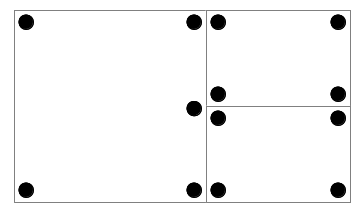
\includegraphics[width=0.3\textwidth]{fig_amr.png}
   %%\caption{Adaptive mesh refinement grid with PWLD finite elements: left cell is interpreted as a pentagon while right cells are quadrangles.}
   %%\label{fig_amr}
%%\end{figure}


%%%%%%%%%%%%%%%%%%%%%%%%%%%%%%%%%%%%%%%%%%%%%%%%%%%%%%%%%%%%%%%%%%%%%%%%%%%%%%%%%%
%\subsection{Rationale for DSA preconditioning}
%%%%%%%%%%%%%%%%%%%%%%%%%%%%%%%%%%%%%%%%%%%%%%%%%%%%%%%%%%%%%%%%%%%%%%%%%%%%%%%%%%

%Next, we recall the rationale for solving transport problems iteratively using 
%diffusion acceleration schemes (preconditioners).
Because analytical solutions are unavailable for most
radiation transport problems of practical interest, one typically employs
iterative techniques to solve the large system of equations that results from
the spatial and angular discretizations of the transport equation. Standard
iterative techniques for the first-order form of the discrete-ordinate (\sn)
transport equation include Source Iteration (SI)  and Krylov 
subspace techniques (usually GMRes \cite{gmres}). For highly diffusive materials 
(i.e., with scattering ratios $c=\Sigma_s / \Sigma_t $ close to 1) and optically 
thick configurations (i.e., problems that are not leakage-dominated), these iterative techniques 
can become quite ineffective, requiring high iteration counts and possibly 
leading to false convergence. To mitigate these issues, SI and GMRes-based transport solves 
can be effectively accelerated (preconditioned) using Diffusion Synthetic Acceleration (DSA) 
\cite{dsa_ref,larsen_dsa,consistent_p1,m4s,wla,mip}. 

The spatial discretization of the DSA equations
must be somewhat ``consistent'' with the one used for the \sn transport equations 
in order to yield unconditionally stable and efficient DSA schemes
\cite{dsa_ref,larsen_dsa,consistent_p1,m4s,wla,mip}. However, the search for full
consistency between the discretized transport equations and the discretized
diffusion may not be computationally practical (especially for unstructured
arbitrary meshes, \cite{dsa_ref}). For instance, Warsa, Wareing, and
Morel \cite{consistent_p1} derived a fully consistent DSA scheme for linear
discontinuous finite elements on unstructured tetrahedral meshes; their DSA
scheme yields a $P_1$ system of equations that is
computationally more expensive than partially consistent DSA schemes that are
based upon discretizations of a standard diffusion equation. Several partially 
consistent schemes have been analyzed for discontinuous finite element
discretizations of the transport equation on unstructured meshes, for
example, the modified-four-step (M4S) scheme \cite{m4s}, the
Wareing-Larsen-Adams (WLA) scheme \cite{wla}, and the Modified Interior
Penalty (MIP) scheme \cite{mip}.

%%%%%%%%%%%%%%%%%%%%%%%%%%%%%%%%%%%%%%%%%%%%%%%%%%%%%%%%%%%%%%%%%%%%%%%%%%%%%%%%%%
%\subsection{PWLD discretization on arbitrary grids}
%%%%%%%%%%%%%%%%%%%%%%%%%%%%%%%%%%%%%%%%%%%%%%%%%%%%%%%%%%%%%%%%%%%%%%%%%%%%%%%%%%

%% Several discretization methods haven been developed for 
%% arbitrary polygonal meshes \cite{pwld_2d,pwld_3d,cfm_dfm,pwl_diffusion,
%% palmer_fe,mimetic,cell_centered_diff,palmer_proc,palmer_ane,wachspress,pwbld}.
%% In this work, we focus on the PWLD discretization because it was successfully
%% used to discretize the transport equation \cite{pwld_2d,pwld_3d}. This
%% discretization can be applied for any polygonal cells and the integrals
%% generated by this discretization can be easily computed analytically. 

To the authors' knowledge, no work is currently ongoing to adapt the M4S 
technique to polygonal meshes. This is very likely due to the fact
that the M4S scheme does not yield a Symmetric Positive Definite (SPD)
matrix and was found to be divergent for 3D tetrahedral meshes with linear 
discontinuous elements \cite{consistent_p1}. 
% 
Recent work to develop a DSA scheme for polygonal cells has mainly focused 
on adapting the WLA scheme to polygonal meshes
\cite{cfm_dfm,wla_pwl}. The WLA scheme is a two-stage process, where first a
diffusion solution is obtained using a {\em continuous} finite element
discretization and then a {\em discontinuous} update is performed cell-by-cell 
in order to provide an appropriate discontinuous scalar flux correction to 
the discontinuous finite element transport 
solver. In \cite{consistent_p1}, the WLA scheme was
found to be a stable and effective DSA technique, though its efficiency
degraded as the problem became optically thick and highly diffusive.
%
In this paper, we extend the MIP technique to the
PWLD discretization technique for arbitrary polygonal meshes.
The MIP scheme is based on the standard Interior Penalty (IP) method for the
discontinuous finite element discretization of diffusion equations. MIP was first derived in
\cite{mip}, where it was applied to triangular unstructured meshes (with
locally adapted cells). MIP does not suffer from the same issues as the WLA technique when the
problem becomes optically thick and highly diffusive and, therefore, can be a
useful alternate DSA for to accelerate DFE transport solves. 
%Because MIP produces an SPD matrix, the authors of \cite{mip}
%have solved the resulting linear system using a Preconditioned Conjugate Gradient (PCG) technique
In \cite{mip}, a Preconditioned Conjugate Gradient (PCG) technique (with Symmetric Gauss-Seidel, 
SGS, as preconditioner) was used to solve the MIP-DSA equation. In this paper, we also analyze  
the effectiveness of algebraic multigrid methods (AMG) \cite{amg,amg_course} as a preconditioner. 
%the MIP-DSA diffusion solve and we compare AMG with PCG. %+\textcolor{red}{SGS/SSOR}.
%Algebraic multigrid methods allow the use of multigrid techniques when no grid
%information is available or when the grid is unstructured. Instead of using a
%succession of grids based on the geometry of the problems, the ``grid levels''
%are based on properties of the matrix.

The remainder of this paper is organized as follows. In Section~\ref {sec_transport},
we briefly review the PWLD discontinuous finite element discretization 
and the iterative solution techniques applied to the 
\sn transport equation. 
The MIP-DSA scheme is extended to the PWLD discretization for arbitrary 
polygons in Section~\ref {sec_mip}. In Section~\ref {sec_amg}, we describe the Algebraic MultiGrid (AMG) 
approaches used here: the ML package of Trilinos \cite{ml_guide} and the
AGMG (AGgregation-based algebraic MultiGrid) technique of 
\cite{agmg_guide,agmg,agmg2,agmg3}. In
Section~\ref {sec_res}, we present a Fourier analysis for the MIP-DSA scheme discretized with
PWLD, and we compare the different preconditioned CG approaches.
Conclusions are given in Section~\ref {sec_conc}.
%%%%%%%%%%%%%%%%%%%%%%%%%%%%%%%%%%%%%%%%%%%%%%%%%%%%%%%%%%%%%%%%%%%%%%%%%%%%%%%%%%%%%%%%%%%%%%%%%%%%%%%%%%%
%%%%%%%%%%%%%%%%%%%%%%%%%%%%%%%%%%%%%%%%%%%%%%%%%%%%%%%%%%%%%%%%%%%%%%%%%%%%%%%%%%%%%%%%%%%%%%%%%%%%%%%%%%%

%%%%%%%%%%%%%%%%%%%%%%%%%%%%%%%%%%%%%%%%%%%%%%%%%%%%%%%%%%%%%%%%%%%%%%%%%%%%%%%%%%%%%%%%%%%%%%%%%%%%%%%%%%%
%%%%%%%%%%%%%%%%%%%%%%%%%%%%%%%%%%%%%%%%%%%%%%%%%%%%%%%%%%%%%%%%%%%%%%%%%%%%%%%%%%%%%%%%%%%%%%%%%%%%%%%%%%%
%%%%%%%%%%%%%%%%%%%%%%%%%%%%%%%%%%%%%%%%%%%%%%%%%%%%%%%%%%%%%%%%%%%%%%%%%%%%%%%%%%
%%%%%%%%%%%%%%%%%%%%%%%%%%%%%%%%%%%%%%%%%%%%%%%%%%%%%%%%%%%%%%%%%%%%%%%%%%%%%%%%%%
\section{Discretization and Solution Techniques for the $S_n$ Transport Equation}\label{sec_transport}
%%%%%%%%%%%%%%%%%%%%%%%%%%%%%%%%%%%%%%%%%%%%%%%%%%%%%%%%%%%%%%%%%%%%%%%%%%%%%%%%%%
%%%%%%%%%%%%%%%%%%%%%%%%%%%%%%%%%%%%%%%%%%%%%%%%%%%%%%%%%%%%%%%%%%%%%%%%%%%%%%%%%%

In this Section, we review the \sn transport equation 
and the iterative solution techniques typically
employed to solve it. 
We then describe the PWLD discontinuous spatial
discretization for the transport equation with an emphasis on arbitrary
polygonal grids.

%%%%%%%%%%%%%%%%%%%%%%%%%%%%%%%%%%%%%%%%%%%%%%%%%%%%%%%%%%%%%%%%%%%%%%%%%%%%%%%%%%
\subsection{The \sn Transport Equations}
%%%%%%%%%%%%%%%%%%%%%%%%%%%%%%%%%%%%%%%%%%%%%%%%%%%%%%%%%%%%%%%%%%%%%%%%%%%%%%%%%%
Given an angular quadrature set $\{\bo _m,w_m\}_{1\leq m \leq M}$, the one-group
\sn transport equation with isotropic source and isotropic scattering is:
%
\begin{equation}
  \( \bo_m\cdot \bn + \Sigma_t(\br) \) \psi_m (\br) = \frac{1}{4\pi} \left( \Sigma_s
  (\br) \phi(\br) + S (\br) \right), \ \textrm{ for } \br \in \mc{D},\
  1 \leq m \leq M,
  \label{transport_sn}
\end{equation}
%
with $\psi_m(\br) = \psi(\br,\bo_m)$ the angular flux at position $\br$ in
direction $\bo_m$, $\Sigma_t$ and $\Sigma_s$ the total and scattering cross
sections, respectively, and $\mc{D}$ the spatial domain. The scalar flux is
defined and numerically evaluated as follows:
%
\begin{equation}
  \phi(\br) \equiv \int_{4\pi} \psi(\br,\bo) d\bo \approx \sum_{m=1}^M w_m
  \psi_m (\br).
\end{equation}
%
For brevity, we assume only incoming boundary conditions, that is, $\psi_m(\br_b) =
\psi_m^{inc}(\br_b)$ for any point on the inflow boundary: $\br_b \in \partial \mc{D}_m^-
= \{\partial \mc{D} \textrm{ such that }\bo_m \cdot \bs{n}_b <0\}$, with
$\bs{n}_b = \bs{n}(\br_b)$ the outward unit normal vector at $\br_b$. 
Equation~\textup {(\ref {transport_sn})} with spatial discretization can be written in a compact form using operators:
%
\begin{align}
  & \bs{L} \Psi = \bs{M \Sigma}\Phi + S \equiv q, \label{L_Psi}\\
  &\Phi = \bs{D} \Psi, \label{Phi}
\end{align}
%
where $\Psi=(\psi_1,\ldots,\psi_M)^T$ is the vector of angular fluxes, $\Phi$ the scalar flux,
$q$ is the total (scattering+external) source, $\bs{L}$ is the streaming plus collision
operator, $\bs{\Sigma}$ is the scattering matrix, $\bs{M}$ is the
moment-to-direction operator, and $\bs{D}$ is the direction-to-moment
operator. $\bs{L} = diag(\bs{L}_1,\hdots,\bs{L}_m,\hdots,\bs{L}_M)$ is 
a block-diagonal operator; given a total source $q$, one can solve independently 
for the resulting angular
fluxes in all directions. The action of $\bs{L}^{-1}$ is often referred to as
a transport sweep when discontinuous spatial approximations are
employed:  for any direction $\bo_m$, the action of $\bs{L}_m^{-1}$ can
be obtained by traversing the mesh (i.e., sweeping) in a specific ordering of
the cells, thus requiring that a small linear system of equations be solved 
cell by cell. The order in which the elements are solved constitutes the graph
of the sweep; for brevity and since this is not the focus of this article,
we do not expand on situations where the graph presents dependencies
(cycles). In such a case, these dependencies can either be lagged within the
iterative procedure \cite{dgfem} or the solution vector consisting of the scalar 
flux is augmented by the angular flux unknowns that cause the cycle \cite{mip}.

%%%%%%%%%%%%%%%%%%%%%%%%%%%%%%%%%%%%%%%%%%%%%%%%%%%%%%%%%%%%%%%%%%%%%%%%%%%%%%%%%%
\subsection{Solution Techniques}
%%%%%%%%%%%%%%%%%%%%%%%%%%%%%%%%%%%%%%%%%%%%%%%%%%%%%%%%%%%%%%%%%%%%%%%%%%%%%%%%%%

Equations~\textup {(\ref {L_Psi})} and~ \textup {(\ref {Phi})} can be solved using the Source Iteration (SI) method (a
stationary iterative technique also known as Richardson iteration). 
The $\ell^{th}$ iteration of SI is given by :
%
\begin{equation}
  \Phi^{(\ell+1)} = \bs{DL}^{-1} \(\bs{M\Sigma}\Phi^{(\ell)} + S\).
\end{equation}
%
Alternatively, a subspace Krylov method (usually GMRes) can be employed to
solve the linear system of equations, recast as follows:
%
\begin{equation}
  \(\bs{I} - \bs{DL}^{-1}\bs{M \Sigma}\) \Phi = \bs{DL}^{-1}S .
\end{equation}
%
SI and GMRes-based transport solves require transport sweeps (the action of $\bs{L}^{-1}$).
When the scattering ratio
$c=\frac{\Sigma_s}{\Sigma_t}$ tends to one in optically thick domains, the
number of SI and GMRes iterations can become large. To speed up convergence, a DSA
preconditioner is needed; this is further discussed in Section~\ref {sec_mip}.

%%%%%%%%%%%%%%%%%%%%%%%%%%%%%%%%%%%%%%%%%%%%%%%%%%%%%%%%%%%%%%%%%%%%%%%%%%%%%%%%%%
\subsection{Discontinuous Finite Element Discretization on Arbitrary Grids}
%%%%%%%%%%%%%%%%%%%%%%%%%%%%%%%%%%%%%%%%%%%%%%%%%%%%%%%%%%%%%%%%%%%%%%%%%%%%%%%%%%

To seek a DFE solution for the angular flux, the domain $\mc{D}$ is partitioned 
into arbitrary polygonal cells. For 
a given streaming direction $\bo_m$, the discontinuous finite
element formulation, on a given spatial cell $K$, is given by:
%
\begin{equation}
  -\int_{K} \(\psi_m \bo_m \cdot \bn \tf + \Sigma_t \Psi_m \tf \)\ d\br +
  \int_{\partial K^+} \bo_m \cdot \bs{n} \Psi_m \tf \ d\br = \int_{K} q\, \tf \ d\br +
  \int_{\partial K^{-}} |\bo_m \cdot \bs{n}| \psi_m^{\uparrow}\, \tf \ d\br,
  \label{transport_int}
\end{equation}
%
where $\tf$ represents a generic discontinuous finite element basis function, $\partial K^{-}$ 
is the inflow face of element $K$, and $\partial K^{+}$ is the outflow face of 
element $K$. The angular flux values on an inflow face, denoted by 
$\psi_m^{\uparrow}$ in Eq.~\textup {(\ref {transport_int})}, are taken from the upwind neighbor 
element of that face.

Next, we define the $\tf$ basis functions for the PWLD discretization. First, we
introduce the within-cell point $c$ for any 2D polygonal cell. The coordinates 
of $c$ are the weighted averages of the polygon's vertices:
%
\begin{equation}
  u_c = \sum_{i=1}^{N_V} \alpha_i u_i,
\end{equation}
%
where $u=x$ or $y$, $N_V$ is the number of vertices for the cell under
consideration, and the (positive) weights $\alpha_i$ are such that $\sum_{i=1}^{N_V} \alpha_i =1$. 
The basis function at vertex $i$ is defined by 
(see also \cite{pwld_2d}):
%
\begin{equation}
  b_i(x,y) = t_i(x,y) + \alpha_i t_c(x,y),
\end{equation}
%
where $t_i(x,y)$ is a linear function such that $t_i(x,y)$ is unity at vertex
$i$ and zero at vertices $i-1$, $i+1$, and $c$. The $t_c(x,y)$ function is a ``tent''
function in the interior of the cell; it is unity at the within-cell point $c$
and zero at all of the vertices of the cell. The number of PWLD basis functions is 
equal to the number of vertices in the polygon (i.e., $1 \le i \le N_V$). In this paper, the arbitrary
positive weights $\alpha_i$ are chosen to be equal to $\frac{1}{N_V}$. For example, on a
quadrilateral cell, we employ $\alpha_i =\frac{1}{4}$. Finally, note that on
triangular cells, the PWLD basis functions reduce to the
standard Linear Discontinuous (LD) basis functions if one chooses $\alpha_i = \frac{1}{3}$. 
Given the definition of the PWLD
finite elements, it may seem complicated to build the elementary transport 
matrices on an arbitrary polygonal cell, but the construction of such matrices
can be greatly simplified using the notion of ``sub-cells'', where a ``sub-cell'',
in 2D, is defined as the triangular cell linking an edge of the polygonal cell to its
within-cell point. Note that these ``sub-cells'' are never created nor stored as part of the 
polygonal grid. However, from a code implementation perspective, the computation of
the elementary matrices on a polygonal cell is greatly simplified by looping over its sub-cells. 

%%%%%%%%%%%%%%%%%%%%%%%%%%%%%%%%%%%%%%%%%%%%%%%%%%%%%%%%%%%%%%%%%%%%%%%%%%%%%%%%%%%%%%%%%%%%%%%%%%%%%%%%%%%
%%%%%%%%%%%%%%%%%%%%%%%%%%%%%%%%%%%%%%%%%%%%%%%%%%%%%%%%%%%%%%%%%%%%%%%%%%%%%%%%%%%%%%%%%%%%%%%%%%%%%%%%%%%

%%%%%%%%%%%%%%%%%%%%%%%%%%%%%%%%%%%%%%%%%%%%%%%%%%%%%%%%%%%%%%%%%%%%%%%%%%%%%%%%%%%%%%%%%%%%%%%%%%%%%%%%%%%
%%%%%%%%%%%%%%%%%%%%%%%%%%%%%%%%%%%%%%%%%%%%%%%%%%%%%%%%%%%%%%%%%%%%%%%%%%%%%%%%%%%%%%%%%%%%%%%%%%%%%%%%%%%
%%%%%%%%%%%%%%%%%%%%%%%%%%%%%%%%%%%%%%%%%%%%%%%%%%%%%%%%%%%%%%%%%%%%%%%%%%%%%%%%%%
%%%%%%%%%%%%%%%%%%%%%%%%%%%%%%%%%%%%%%%%%%%%%%%%%%%%%%%%%%%%%%%%%%%%%%%%%%%%%%%%%%
\section{Diffusion Synthetic Acceleration (DSA) on Arbitrary Polygonal Cells} \label{sec_mip}
%%%%%%%%%%%%%%%%%%%%%%%%%%%%%%%%%%%%%%%%%%%%%%%%%%%%%%%%%%%%%%%%%%%%%%%%%%%%%%%%%%
%%%%%%%%%%%%%%%%%%%%%%%%%%%%%%%%%%%%%%%%%%%%%%%%%%%%%%%%%%%%%%%%%%%%%%%%%%%%%%%%%%

%%%%%%%%%%%%%%%%%%%%%%%%%%%%%%%%%%%%%%%%%%%%%%%%%%%%%%%%%%%%%%%%%%%%%%%%%%%%%%%%%%
\subsection{DSA Solution Principle}
%%%%%%%%%%%%%%%%%%%%%%%%%%%%%%%%%%%%%%%%%%%%%%%%%%%%%%%%%%%%%%%%%%%%%%%%%%%%%%%%%%

As noted earlier, standard iterative techniques applied to transport solves 
can be slowly converging in thick diffusive configurations. A DSA scheme 
must be employed to accelerate their convergence.
The idea behind synthetic acceleration is that the error between the (yet
unknown) transport solution and the current iterate can be estimated from a
computationally less expensive process, yielding a corrective term to be added
to the current iterate in order to improve the next iterate. In DSA, a
corrective scalar flux contribution, $\delta \Phi$, is sought through the following 
diffusion equation \cite{dsa_ref}, 
%
\begin{equation}
  \bs{A}\ \delta \Phi = \bs{\Sigma}\(\Phi^{(\ell+1/2)} - \Phi^{(\ell)}\).
\end{equation}
%
where the source term is a scattering term due to the
difference between the previous iterate scalar flux $\Phi^{(\ell)}$ and the
newest scalar flux, $\Phi^{(\ell+1/2)}$, obtained after a single transport sweep. 
The next scalar flux iterate is obtained by adding the scalar flux correction to
the latest scalar flux, yielding:
%
\begin{equation}
  \Phi^{(\ell+1)} = \Phi^{(\ell+1/2)}+\delta \Phi.
\end{equation}
%
$\bs{A}$ is the diffusion matrix of the DSA scheme.
Ideally, $\bs{A}$ should be SPD (such that efficient iterative techniques can 
be employed in its linear solve) and easy to form (even on arbitrary grids).

%%%%%%%%%%%%%%%%%%%%%%%%%%%%%%%%%%%%%%%%%%%%%%%%%%%%%%%%%%%%%%%%%%%%%%%%%%%%%%%%%%
\subsection{Modified Interior Penalty DSA Scheme for Polygons}
%%%%%%%%%%%%%%%%%%%%%%%%%%%%%%%%%%%%%%%%%%%%%%%%%%%%%%%%%%%%%%%%%%%%%%%%%%%%%%%%%%

Here, we discuss the Modified Interior Penalty (MIP) method for the diffusion equation for arbitrary polygons
as a DSA scheme. 
In its discretization, this DSA scheme employs the same discontinuous finite elements used in the 
discretization of the transport operator. 
MIP as a DSA scheme has been shown to be always stable on triangular cells for isotropic scattering \cite{mip}
(for highly forward-peaked scattering, DSA is not an efficient preconditioner and one needs to employ
an angular multigrid technique \cite{angular_multigrid_1d}, whose coarsest angular level can be a diffusion solve;
see \cite{angular_multigrid_bruno} for instance). 
The MIP diffusion solve is based on the standard Interior Penalty (IP) method
\cite{Kanschat2007}.
%, with an \textcolor{red}{appropriately modified} penalty term. 
Consider the following diffusion update equation:
%
\begin{align}
  \label{eq:dsa}
  \left(-\bn \cdot \mathrm{D} \bn  + \Sigma_a \right) \delta \phi &= Q_0 &\textrm{ for }\br \in
  \mc{D}\\
  \label{eq:dsa-bc}
  \frac{1}{4}\delta \phi - \frac{1}{2} \mathrm{D} \partial_n \delta \phi & = 0 &\textrm{ for }
  \br \in \partial \mc{D} %^d \\
  %-\mathrm{D} \partial_n \phi &= J^{inc} & \textrm{ for } \br \in \partial
  %\mc{D}^r,
\end{align}
%
where $\mathrm{D}$ is the diffusion coefficient and $\Sigma_a$ is the absorption cross section. 
%
%$\partial \mc{D}^d$ is the
%boundary of the domain with Dirichlet condition, $\partial \mc{D}^r$ is the
%boundary of the domain with reflective condition, 
%
For DSA, the volumetric source term is given by the scattering due to the difference in scalar flux
between two iterations, $Q_0=\Sigma_s\(\Phi^{(\ell+1/2)}-\Phi^{(\ell)}\)$, 
%
%$J^{inc} = \sum_{\bo_m\cdot\bs{n}_b >0} w_m 
%|\bo_m \cdot \bs{n}_b| \delta \psi_d$, 
%
and the known incoming angular flux boundary condition from the transport problem translates into the Robin-type
vacuum boundary condition given in Equation~\textup {(\ref {eq:dsa-bc})}, where $\partial_{n} = \bs{n}\cdot \bn$
and $\bs{n}$ is the outer normal unit vector on the domain's boundary, $\partial \mc{D}$. 
%
%where
%$\bs{n}_e$ is the normal unit vector associated with a given edge $e$ (on the
%boundary $\bs{n}_e = \bs{n}_b$). 
%The only difference between IP and MIP is the
%penalty factor $\kappa_e^{IP}$ used for IP is replaced by a new penalty factor
%$\kappa_e^{MIP}$. Therefore, 
%
The MIP weak form for the DSA update equation is given by:
\begin{equation}
a(\delta \phi,\phi^*) = l(\phi^*)
\label{mip}
\end{equation}
%
with the bilinear (matrix) form:
\begin{equation}
\begin{split}
a(\delta \phi,\phi^*) =& \(\Sigma_a \delta \phi,\phi^*\)_{\mc{D}}
  + (\mathrm{D}\bn\delta \phi,\bn\phi^*)_{\mc{D}} 
	+ \( \kappa_e^{MIP} \jmp{\delta \phi}, \jmp{\phi^*}      \)_{E_h^i} 
	+ \( \jmp{\delta \phi}, \mvl{\mathrm{D}\partial_n\phi^*} \)_{E_h^i} \\	
& + \( \mvl{\mathrm{D}\partial_n \delta \phi},\jmp{\phi^*} \)_{E_h^i} 
  + \(\kappa_e^{MIP} \delta \phi,\phi^*\)_{\partial \mc{D}^d} 
	- \frac{1}{2} \(\delta \phi,\mathrm{D} \partial_n\phi^*\)_{\partial \mc{D}^d} 
	- \frac{1}{2} \(\mathrm{D} \partial_n\delta \phi,\phi^*\)_{\partial \mc{D}^d}
\label{mip_b}
\end{split}
\end{equation}
%
and the linear (right-hand-side) form
%
\begin{equation}
l(\phi^*) = (Q_0,\phi^*)_{\mc{D}}\ . % + (J^{inc},\phi^*)_{\partial \mc{D}^r} .
\label{mip_l}
\end{equation}
%
The notations used are as follows:
the domain integral is split onto the element integrals, $(f,g)_{\mc{D}} = \sum_{K\in \mathbb{T}_h} \(f,g\)_K$, with the element integrals defined as 
$(f,g)_K = \int_K fg\ d\br$; and 
the integral over all interior edges is $(f,g)_{E_h^i}=\sum_{e\in E_h^i}(f,g)_e$, with the edge integrals defined as 
$(f,g)_e = \int_e fg\ ds$. In the above, 
 $\mathbb{T}_h$ denotes the partition of domain
$\mc{D}$ into non-overlapping elements $K$, $E_h^i$ is the set of interior
edges, $\delta \phi$ is the numerical solution for the diffusion correction, and $\phi^*$ is any test function.
Any entry $A_{ij}$ of matrix $\bs{A}$ is simply given by $A_{ij}= a(b_j,b_i)$. The resulting matrix $\bs{A}$ is SPD
\cite{Arnold1982,arnold2000discontinuous} and thus can be solved using a preconditioned conjugate gradient technique.
%
%$\in W_{\mc{D}}^h$, $W_{\mc{D}}^h=\{P \in
%L^2(\mc{D}); P|_{K}\in V_p(K), \forall K \in \mathbb{T}_h\}$, where $V_p(K)$
%is the space of polynomials of degree up to $p$ on element $K$,  
%
The jump and mean value of a variable $u$  at the interface between two elements is defined as follows:
%
\begin{equation}
\jmp{u} = u^+ - u^- \text{ and } \mvl{u} = \frac{u^+ + u^-}{2} ,
\end{equation}
respectively.
%
The definition of the left/right values along a given edge $e$ is
%
\begin{equation}
u^{\pm}= \lim_{s\rightarrow 0^{\pm}}u(\bs{r}+s\bs{n}_e) ,
\end{equation}
%
where $\bs{n}_e$ is the normal unit vector associated with the given edge $e$
(on the boundary $\bs{n}_e$ is the external normal).
%
The MIP penalty coefficient is given by
%
\begin{equation}
\kappa_e^{MIP} = \max\(\kappa_e^{IP},\frac{1}{4}\)
\end{equation}
with:
\begin{equation}
\kappa_e^{IP} = \left\{
\begin{aligned}
&\frac{c}{2} \left( \frac{\mathrm{D^+}}{h_{\bot}^+} + \frac{\mathrm{D}^-}{h_{\bot}^-} \right) & \textrm{on interior edges, i.e., for }
e\in E_h^i\\
&c \frac{\mathrm{D}}{h_{\bot}} & \textrm{on boundary edges, i.e., for } e
\in\partial \mc{D} %^d 
\end{aligned}
\right. 
\end{equation}
%
where $c$ is a constant (chosen equal to 4 here) and $h_{\bot}$ is the length of the cell in the direction
orthogonal to the edge $e$. 
%
%MIP yields only a correction for the scalar flux
%but by assuming that the angular dependence satisfies a diffusion expansion,
%the angular correction can be computed using:
%\begin{equation}
  %\varepsilon_d = \frac{1}{4\pi}(\phi-3\mathrm{D}\bn\phi\cdot \bo_d)
%\end{equation}
%This correction can be used when some of the boundary conditions are periodic
%or reflective.
%
When polygonal cells are employed, there are no 
simple ways in which to compute $h_{\bot}$. To estimate $h_{\bot}$, we 
assume that the polygonal cells do not deviate significantly from regular polygons. 
In such cases, if the regular polygon has an even number of edges, the orthogonal 
length equals two times the apothem. The apothem is the line segment between the 
polygon's center and the midpoint of the polygon's side and its length is equal to
twice the polygon's area divided by the polygon's perimeter,
$\textrm{apothem}=2\times \tfrac{\textrm{area}}{\textrm{perimeter}}$. 
If polygon has an odd number of sides, its orthogonal length is given by the sum of the
apothem and the circumradius, the latter being the radius of the circle circumscribed to 
the polygon $\(\textrm{circumradius}=\sqrt{\tfrac{2\times \textrm{area}}{N_V
\sin\(\frac{2\pi}{N_V}\)}}\)$. A summary of the definitions used for $h_{\bot}$ for 
any polygon as a function of the number of vertices is given in
Table~\ref {table_h_bot}.
%
\begin{table}[H]
  \begin{center}
    \caption{Orthogonal length $h_{\bot}$ for different polygonal types : 
		$\textrm{area}$ is the polygon's area; $\textrm{perimeter}$ is the polygon's perimeter; 
		$N_V$ is the number of vertices; $L_e $ is the edge's length.}
    \begin{tabular}{|c|c|c|c|c|}
      \hline
      Number of vertices & 3 & 4 & $> 4$ and even & $> 4$ and odd \\
      \hline
      $h_{\bot}$ & $2 \times \frac{\textrm{area}}{L_e}$ &
$\frac{\textrm{area}}{L_e}$ & $4\times
\frac{\textrm{area}}{\textrm{perimeter}}$ & $2 \times
      \frac{\textrm{area}}{\textrm{perimeter}}+\sqrt{\frac{2\times
      \textrm{area}}{N_V\sin\(\frac{2\pi}{N_V}\)}}$\\
      \hline
    \end{tabular}
    \label{table_h_bot}
  \end{center}
\end{table}
%%%%%%%%%%%%%%%%%%%%%%%%%%%%%%%%%%%%%%%%%%%%%%%%%%%%%%%%%%%%%%%%%%%%%%%%%%%%%%%%%%%%%%%%%%%%%%%%%%%%%%%%%%%
%%%%%%%%%%%%%%%%%%%%%%%%%%%%%%%%%%%%%%%%%%%%%%%%%%%%%%%%%%%%%%%%%%%%%%%%%%%%%%%%%%%%%%%%%%%%%%%%%%%%%%%%%%%

\textcolor{red}{elementary matrices}

%%%%%%%%%%%%%%%%%%%%%%%%%%%%%%%%%%%%%%%%%%%%%%%%%%%%%%%%%%%%%%%%%%%%%%%%%%%%%%%%%%%%%%%%%%%%%%%%%%%%%%%%%%%
%%%%%%%%%%%%%%%%%%%%%%%%%%%%%%%%%%%%%%%%%%%%%%%%%%%%%%%%%%%%%%%%%%%%%%%%%%%%%%%%%%%%%%%%%%%%%%%%%%%%%%%%%%%
%%%%%%%%%%%%%%%%%%%%%%%%%%%%%%%%%%%%%%%%%%%%%%%%%%%%%%%%%%%%%%%%%%%%%%%%%%%%%%%%%%
%%%%%%%%%%%%%%%%%%%%%%%%%%%%%%%%%%%%%%%%%%%%%%%%%%%%%%%%%%%%%%%%%%%%%%%%%%%%%%%%%%
\section{MIP-DSA Solves Based on Algebraic Multigrid Techniques} \label{sec_amg}
%%%%%%%%%%%%%%%%%%%%%%%%%%%%%%%%%%%%%%%%%%%%%%%%%%%%%%%%%%%%%%%%%%%%%%%%%%%%%%%%%%
%%%%%%%%%%%%%%%%%%%%%%%%%%%%%%%%%%%%%%%%%%%%%%%%%%%%%%%%%%%%%%%%%%%%%%%%%%%%%%%%%%

%%%%%%%%%%%%%%%%%%%%%%%%%%%%%%%%%%%%%%%%%%%%%%%%%%%%%%%%%%%%%%%%%%%%%%%%%%%%%%%%%%
\subsection{AMG Principles}
%%%%%%%%%%%%%%%%%%%%%%%%%%%%%%%%%%%%%%%%%%%%%%%%%%%%%%%%%%%%%%%%%%%%%%%%%%%%%%%%%%

A common way to solve an SPD system of equations is to use a 
Conjugate Gradient (CG) technique preconditioned  with Symmetric Gauss-Seidel (PCG-SGS)
or SSOR (PCG-SSOR); SGS is simply SSOR with a damping factor of one. Here, we
compare CG preconditioned with Symmetric Gauss-Seidel (PCG-SGS) with CG preconditioned with an
algebraic multigrid method. PCG-SGS was chosen because little difference was noted 
when employing other damping factors for MIP-DSA on triangular grids \cite{wang_personal_comm}. 
%An algebraic multigrid method was employed to precondition the Krylov solver for the 
%even-parity finite element-spherical harmonics (FE-$P_N$) method; see, for instance,
%\cite{amg_pn}. In \cite{amg_pn}, the use of AMG  as a 
%preconditioner resulted in a 60\% reduction in the solution time compared to 
%ILU(0) preconditioning and even more reduction compared to SSOR preconditioning. 
In our implementation, we have linked our code with the ML package 
\cite{ml_guide} of the Trilinos library and with the AGMG library \cite{agmg_guide}. 
ML is a multigrid preconditioning package that uses a smoothed aggregation 
algebraic multigrid to build a preconditioner for a Krylov method. AGMG is an 
aggregation-based algebraic multigrid library written in Fortran 90.
%
The first multigrid methods developed were geometric multigrid techniques, used as 
stand-alone solvers. In many applications, they achieve the so-called 
``textbook multigrid efficiency'', i.e., ``the solution to the governing 
system of equations [is attained] in a computational work that is a small 
multiple of the operation counts associated with discretizing the system'' 
\cite{textbook_eff}. However, in many other applications, multigrid methods, 
and particularly algebraic multigrid methods, may not achieve such efficiency, 
\cite{k_cycle} and, in such cases, they are often used as preconditioner for 
Krylov subspace methods. 

Before describing a general multigrid method, we recall the process using 
two grids. Consider the following system
\begin{equation}
  \bs{A}_f u_f = b_f,
\end{equation}
defined on a fine grid $\Gamma_f$. The two-grid algorithm is as follows:
\begin{enumerate}
  \item Perform $\nu_1$ pre-smoothing iterations using a smoother (Jacobi,
    Gauss-Seidel, or ILU) and an initial guess $u_0$: $u = S^{\nu_1}(u_0,b_f)$
  \item Compute the residual on the fine grid $\Gamma_f$ and restrict it to
    the coarse grid $\Gamma_c$: $r_c = \bs{R}(b_f-\bs{A}_f u)$;
  \item Solve the system on the coarse grid: $v=\bs{A}_c^{-1} r_c$;
  \item Interpolate the coarse grid correction to the fine grid and add the
    correction to $u$: $u \leftarrow u+\bs{P}v$;
  \item Perform $\nu_2$ post-smoothing iterations: $u = S^{\nu_2}(u,b_f)$.
\end{enumerate}
When using AMG, the matrix $\bs{A}_c$ on the coarse grid is given by the
Galerkin approximation:
\begin{equation}
  \bs{A}_c = \bs{R} \bs{A}_f \bs{P},
\end{equation}
where $\bs{P}$ is a prolongation matrix and $\bs{R}$ is a restriction matrix. 
Generally, solving the system $\bs{A}_c v = r_c$ on the coarse grid is still
quite expensive, therefore this step is recursively replaced by $n_{\gamma}$
sequences of the two-grid method until the system can be efficiently inverted 
with a direct solver.
%This yields the multigrid method. 
When $n_\gamma = 1$, respectively $n_\gamma =
2$, the multigrid method is said to use a $V-$cycle, respectively a $W-$cycle. 
Figure~\ref {fig_v_w} shows typical $V-$ and $W-$ cycles. In Figure~\ref {fig_v_w}, a 
dot represents a smoothing operation and a square a
direct inversion; the grid transfer operators are symbolized by the line segments.
\begin{figure}[H]
  \centering
  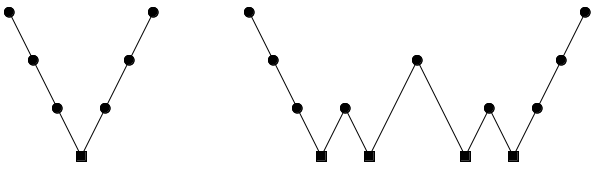
\includegraphics[width=0.5\textwidth]{v_w_cycles}
  \caption{$V-$ and $W-$cycles.}
  \label{fig_v_w}
\end{figure}

The main difference between geometric and algebraic multigrid techniques
lies in the method used
to coarsen the grid. Algebraic multigrid methods only use the properties of the
matrix. Among the algebraic multigrid methods, there are three main categories: 
the classical Ruge-Stueben AMG, the plain aggregation AMG, and the
smoothed aggregation AMG. ML uses smoothed aggregation AMG and AGMG
uses plain aggregation AMG. Next, we briefly explain the coarsening step in
the ML and AGMG implementations. The coarsening step is a crucial step 
because convergence rates will decrease if coarsening occurs too quickly. 
However, if coarsening is too slow, more memory may be required to solve the problem. 

%%%%%%%%%%%%%%%%%%%%%%%%%%%%%%%%%%%%%%%%%%%%%%%%%%%%%%%%%%%%%%%%%%%%%%%%%%%%%%%%%%
\subsection{The ML Package of Trilinos}
%%%%%%%%%%%%%%%%%%%%%%%%%%%%%%%%%%%%%%%%%%%%%%%%%%%%%%%%%%%%%%%%%%%%%%%%%%%%%%%%%%
When using a smoothed aggregation scheme, the smoothed interpolation operators
$\bs{P}_k$ are the transpose of the coarsening operators
$\bs{R}_k=\bs{P}_k^T$. Therefore, when the $\bs{P}_k$ matrices are built, the
coarsening operator is also known. First, the graph of the matrix is
constructed: if element $(i,j)$ or $(j,i)$ of the matrix is non-zero, an edge
is built between the vertex $i$ and the vertex $j$ \cite{ml_guide}. Second,
the vertices are 
aggregated. When using ML on a single processor, two aggregation schemes can
be used: the uncoupled scheme or the maximally independent sets (MIS) scheme. 
The uncoupled scheme tries to build aggregates of size $3^d$ where $d$ is the
dimension of the problem; its algorithm proceeds as follows \cite{mis}:
\begin{description}
  \item[Step 1:] As long as there are points not adjacent to an aggregate:
    \begin{enumerate}
      \item Choose a point which is not an adjacent to an
        aggregate. This point is a new root point.
      \item Define a new aggregate as the root point and its neighbors .
    \end{enumerate}
  \item[Step 2:] Add all the points left to the existing aggregates or form 
    new aggregates with them.
\end{description}
The MIS scheme used in ML applies the MIS algorithm \cite{graph_coloring} to
the graph of the matrix $\bs{A}^2$. These two coarsening 
schemes use a fixed ratio of coarsening between levels. 
%
Once the aggregation is done, a tentative prolongation matrix, $\bs{\tilde{P}}_k$ 
is constructed \cite{mis}. A example of $\bs{\tilde{P}}_k$ is given by:
\begin{equation}
  \bs{\tilde{P}}_k(i,j) = \left\{
  \begin{aligned}
    &1 &\textrm{if the }i^{th}\textrm{ point is contained in the }j^{th}\textrm{
    aggregate}\\
    & 0 &\textrm{otherwise}
  \end{aligned}
  \right.
\end{equation}
This tentative prolongation operator could be used as is but smoothing it
allows to have a more robust scheme. Let $\bs{S}_k$ be a smoother, for example
damped Jacobi. Then, the prolongation matrix is given by:
\begin{equation}
  \bs{P}_k = \bs{S}_k \bs{\tilde{P}}_k.
\end{equation}

%%%%%%%%%%%%%%%%%%%%%%%%%%%%%%%%%%%%%%%%%%%%%%%%%%%%%%%%%%%%%%%%%%%%%%%%%%%%%%%%%%
\subsection{The AGMG Package}
%%%%%%%%%%%%%%%%%%%%%%%%%%%%%%%%%%%%%%%%%%%%%%%%%%%%%%%%%%%%%%%%%%%%%%%%%%%%%%%%%%
Unlike ML, the prolongation operator in AGMG is not smoothed; this results in a
cheaper setup and a decrease in memory requirements \cite{agmg2}. However,
such a scheme could be less robust. To counteract this weakness, the
aggregation scheme is more involved. Coarsening algorithms that control
the size of the aggregates tend to produce a few badly shaped aggregates.
Since the convergence of AMG is bounded by the worst aggregate, even a small 
number of badly shaped aggregates can have a huge impact on
the convergence. In AGMG, the aggregation algorithm has as input the upper
bound of the two-grid condition number. When the aggregates are constructed,
their quality is checked. This increases the cost of the coarsening
and therefore, it is important that the coarsening is fast enough. Such an 
algorithm does not control the size of the aggregates, and, therefore, it is 
difficult to control the speed of coarsening. However, controlling the condition 
number rather than the coarsening speed can be an effective alternative approach. By 
monitoring the condition number, bad aggregates will not be created and, instead, 
a few aggregates below the target size may be generated. This  
does not affect the efficiency of the method in a noticeable way \cite{agmg2}. 
A simple way to create the aggregates would be to try to exhaust all of the possible 
combinations, compute their quality, and then choose the optimal
coarsening. In practice, this would be too costly, and, in AGMG, the aggregation 
step is done by a few passes of a pairwise aggregation algorithm. Each pass
aggregates the variables two by two to allow a simple computation of the aggregate 
quality and to keep the cost per iteration low. 
%%The advantage of controlling the 
%%condition number becomes even more important when a $K-$cycle, or Krylov-cycle, is 
%%used instead of the more common $V-$ or $W-$cycles. The difference between the 
%%$K-$cycle and the $V-$ or $W-$cycles is that $K-$cycles use a 
%%few iterations of a Krylov solver preconditioned by a coarser grid to solve 
%%the coarse grid problem in the two-grid algorithm \cite{k_cycle}. The
%%advantage of the $K-$cycle is an increased robustness compared to $V-$ and
%%$W-$cycle. This scheme 
%%is nonlinear and requires, when the system is SPD, the use of flexible CG 
%%\cite{fcg,fcg_2,fcg_3,fcg_4} as the Krylov solver. Even when the condition 
%%number of the two-grid method is large, the convergence properties of the 
%%$K-$cycle can be independent of the number of levels \cite{k_cycle}. The 
%%computational cost of the $K-$cycle is about the same than that of a $W-$cycle. 
%%If the number of unknowns does not decrease sufficiently from one 
%%level to the next, the $K-$cycle at one level is replaced by a $V-$cycle at 
%%this level. At that level, no Krylov solver is used in order to decrease the
%%computational cost of the method. 

%\textcolor{red}{so what is used?}
%%%%%%%%%%%%%%%%%%%%%%%%%%%%%%%%%%%%%%%%%%%%%%%%%%%%%%%%%%%%%%%%%%%%%%%%%%%%%%%%%%%%%%%%%%%%%%%%%%%%%%%%%%%
%%%%%%%%%%%%%%%%%%%%%%%%%%%%%%%%%%%%%%%%%%%%%%%%%%%%%%%%%%%%%%%%%%%%%%%%%%%%%%%%%%%%%%%%%%%%%%%%%%%%%%%%%%%

%%%%%%%%%%%%%%%%%%%%%%%%%%%%%%%%%%%%%%%%%%%%%%%%%%%%%%%%%%%%%%%%%%%%%%%%%%%%%%%%%%%%%%%%%%%%%%%%%%%%%%%%%%%
%%%%%%%%%%%%%%%%%%%%%%%%%%%%%%%%%%%%%%%%%%%%%%%%%%%%%%%%%%%%%%%%%%%%%%%%%%%%%%%%%%%%%%%%%%%%%%%%%%%%%%%%%%%
%%%%%%%%%%%%%%%%%%%%%%%%%%%%%%%%%%%%%%%%%%%%%%%%%%%%%%%%%%%%%%%%%%%%%%%%%%%%%%%%%%
%%%%%%%%%%%%%%%%%%%%%%%%%%%%%%%%%%%%%%%%%%%%%%%%%%%%%%%%%%%%%%%%%%%%%%%%%%%%%%%%%%
\section{Numerical Results} \label{sec_res}
%%%%%%%%%%%%%%%%%%%%%%%%%%%%%%%%%%%%%%%%%%%%%%%%%%%%%%%%%%%%%%%%%%%%%%%%%%%%%%%%%%
%%%%%%%%%%%%%%%%%%%%%%%%%%%%%%%%%%%%%%%%%%%%%%%%%%%%%%%%%%%%%%%%%%%%%%%%%%%%%%%%%%

In this section, we present two series of results. First, Fourier analyses are 
carried out to analyze the performance of the MIP-DSA acceleration scheme 
for an homogeneous infinite medium meshed with rectangular cells and discretized with PWLD finite elements.
The effects of the $S_n$ order and the cell aspect ratio on the spectral radius of the iterative 
scheme are also studied. Second, the MIP-DSA technique is implemented in a 2D \sn code that uses
arbitrary polygonal grids with a PWLD spatial discretization.  Numerical examples employ
several mesh types: arbitrary quadrilaterals; arbitrary polygons; a grid containing a regular layout of 
hexagons/triangles/rectangles; and a grid that mimics adaptive mesh refinement 
performed on rectangular cells. The MIP-DSA diffusion solves are performed using various
linear solvers: Conjugate Gradient (CG); Conjugate Gradient
Preconditioned with Symmetric Gauss-Seidel (PCG-SGS); Conjugate Gradient
Preconditioned with ML using Uncoupled aggregation (PCG-ML/U);
Conjugate Gradient Preconditioned with ML using MIS aggregation (PCG-ML/MIS);
and Conjugate Gradient Preconditioned with AGMG (AGMG). 

%%%%%%%%%%%%%%%%%%%%%%%%%%%%%%%%%%%%%%%%%%%%%%%%%%%%%%%%%%%%%%%%%%%%%%%%%%%%%%%%%%
\subsection{Fourier Analyses}
%%%%%%%%%%%%%%%%%%%%%%%%%%%%%%%%%%%%%%%%%%%%%%%%%%%%%%%%%%%%%%%%%%%%%%%%%%%%%%%%%%

Fourier analysis is often performed to assess some of the properties of 
DSA-accelerated transport solves \cite{dsa_ref,larsen_dsa,consistent_p1}. In a Fourier analysis,
the eigenvalues of the iteration matrix are analyzed, assuming a Fourier ansatz for the 
error modes. Specifically, the iteration matrices for the SI and SI+DSA schemes are given by
\begin{equation}
\bs{D L^{-1}M \Sigma} \quad \text{and} \quad \bs{I}-\bs{(I+A^{-1}\Sigma)(I-D L^{-1}M \Sigma)},
\end{equation}
respectively.  The error modes are of the form $\exp(i \bs{\Lambda} \cdot \bs{r})$ with the
wave number $\bs{\Lambda}=[\lambda_x,\, \lambda_y]^T$. This expression for the error modes 
is inserted into the discretized equations and the spectral radius (largest eigenvalue in magnitude)
of the iteration matrices are sought for $0 \le \lambda_x \le 2\pi/X$ and $0 \le \lambda_y \le 2\pi/Y$,
where $X$ and $Y$ are the dimensions of the rectangular domain.


\subsubsection{Spectral Radius as a Function of the $S_n$ Order}
%%%%%%%%%%%%%%%%%%%%%%%%%%%%%%%%%%%%%%%%%%%%%%%%%%%%%%%%%%%%%%%%%%%%%%%%%%%%%%%%%%

This Fourier analysis is carried on a square cell ($X=Y$) using a triangular 
Gauss-Legendre-Chebyshev (GLC) angular quadrature \cite{quadrature}. The medium is homogeneous with a 
scattering ratio $c=0.9999$; periodic boundary conditions are used. The results 
are plotted on Figure~\ref {fig_fa_sn}, where the $x-$axis is the mesh size in mean free 
paths and the $y-$axis is the spectral radius. There are four curves corresponding 
to different $S_n$ orders: $S_2$, $S_4$, $S_8$, and $S_{16}$.
From Figure~\ref {fig_fa_sn}, we conclude that a PWLD discretization of the MIP-DSA equations 
is stable for every cell size. The spectral radius is always less than 0.5, except for $S_2$ where 
it is about 0.7. In the fine mesh limit, the continuum results are recovered \cite{multisweep}. Notably,
the spectral radius of SI+DSA using an $S_2$ quadrature in 2D undiscretized space is $0.5c$. Also, as the angular 
quadrature is refined, the standard limit value of $0.2247c$ for the spectral result is reached.
\begin{figure}[!htbp]
  \centering
  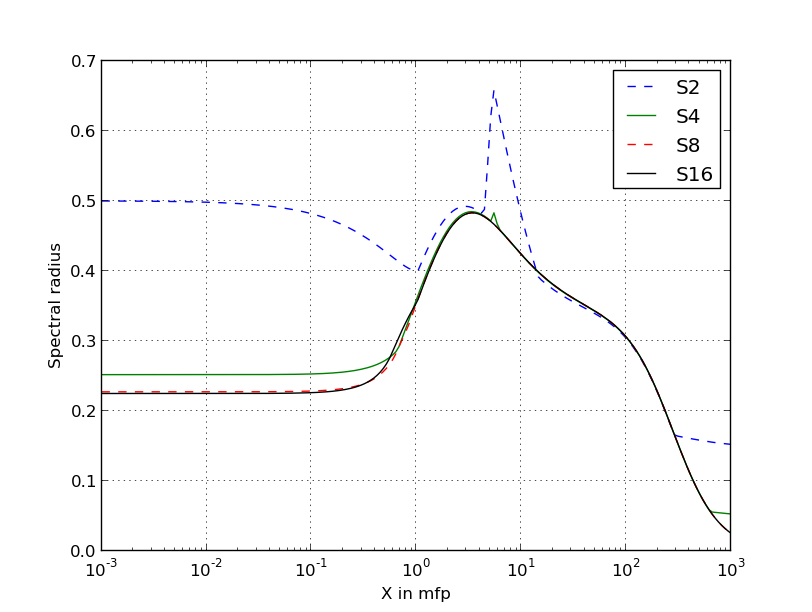
\includegraphics[width=0.7\textwidth]{sn_order_9999}
  \caption{Spectral radius as a function of the mesh optical thickness for various \sn orders (Fourier analysis on a square cell).}
  \label{fig_fa_sn}
\end{figure}

\subsubsection{Spectral Radius as a Function of the Cell Aspect Ratio}
%%%%%%%%%%%%%%%%%%%%%%%%%%%%%%%%%%%%%%%%%%%%%%%%%%%%%%%%%%%%%%%%%%%%%%%%%%%%%%%%%%
For this Fourier analysis, we use a $S_{16}$ GLC quadrature. The medium is
again homogeneous with $c=0.9999$, and periodic boundary conditions apply. 
On Figure~\ref {fig_fa_ar}, the five curves correspond to the following cell aspect 
ratios: $\frac{Y}{X}=\frac{1}{16}$; $\frac{1}{4}$;
$1$; $4$; $16$; and $100$.
We note that the MIP-DSA scheme is stable for every aspect ratio tested, including an
aspect ratio value of 100, 
and that the maximum spectral radius shows little sensitivity to the aspect ratio.
\begin{figure}[!htbp]
  \centering
  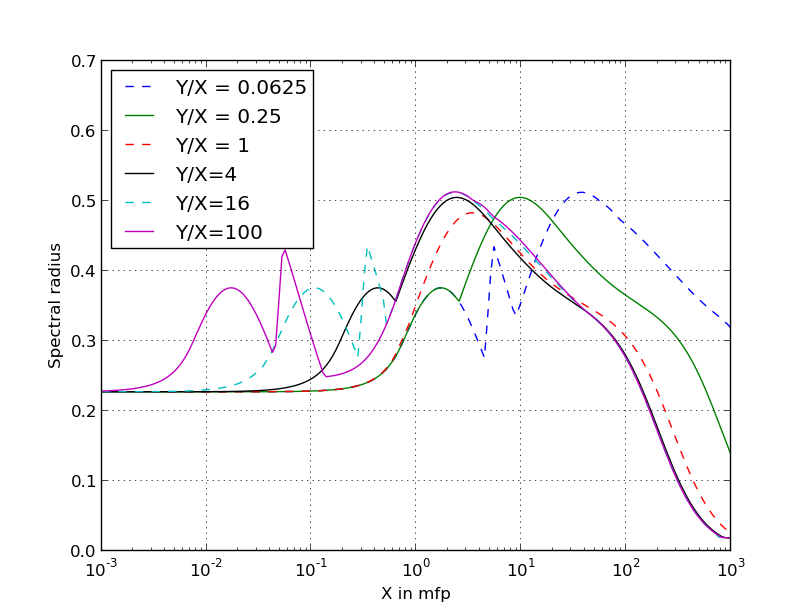
\includegraphics[width=0.7\textwidth]{aspect_ratio_9999_2}
  \caption{Spectral radius as a function of the mesh optical thickness for various cell aspect ratios (Fourier analysis carried out using an $S_{16}$ angular quadrature).}
  \label{fig_fa_ar}
\end{figure}

%%%%%%%%%%%%%%%%%%%%%%%%%%%%%%%%%%%%%%%%%%%%%%%%%%%%%%%%%%%%%%%%%%%%%%%%%%%%%%%%%%
\subsection{Performance of MIP-DSA Implemented in a PWLD $S_n$ Transport Code}
%%%%%%%%%%%%%%%%%%%%%%%%%%%%%%%%%%%%%%%%%%%%%%%%%%%%%%%%%%%%%%%%%%%%%%%%%%%%%%%%%%
The MIP-DSA scheme has been implemented in a 2D \sn code that employs a PWLD discretization
for arbitrary polygonal grids. Several test cases are presented.

\subsubsection{Homogeneous Test Cases}  \label{sec_homog}
%%%%%%%%%%%%%%%%%%%%%%%%%%%%%%%%%%%%%%%%%%%%%%%%%%%%%%%%%%%%%%%%%%%%%%%%%%%%%%%%%%

We compare the different linear solvers employed for MIP-DSA using a homogeneous medium, $100cm
\times 100cm$, $\Sigma_t = 1cm^{-1}$ and $\Sigma_s = 0.999cm^{-1}$, with
vacuum boundary conditions and a unit source of intensity $1cm^{-3}s^{-1}$. We
use an $S_8$ angular quadrature. A relative tolerance of  $10^{-8}$ is used for the Source Iteration solver
while the MIP-DSA solvers employs a relative tolerance of $10^{-10}$. 
The domain is discretized using two different meshes:
\begin{enumerate}
  \item A quadrilateral grid composed of 49263 quadrilateral
    cells (197,052 degrees of freedom or spatial unknowns per angular direction). This grid was 
		obtained from an unstructured triangular grid in which each triangle was split into 3 quadrangles.
  \item A polygonal grid composed of 45,204 triangles, 823
    quadrilaterals, 4,978 pentagons, 4,155 hexagons, 725 heptagons, and 24
    octagons, for a total of 55,909 cells and 193,991 degrees of freedom. This grid was obtained 
		from the same triangular grid as before. This time, vertices were removed and the triangles 
		containing them were merged into polygons. Since an arbitrary number of triangles may contain 
		a given point, deleting a vertex leads to various polygonal types. This
    example allows us to test MIP and the different preconditioners on a
    mesh composed of different cell types.
\end{enumerate}
%
The meshes and the numerical solutions are given in Figures~\ref {homog_test_quads} and~ \ref {homog_test_polys}.
In Table~\ref {comparison_homog_quad}, results obtained with the different linear solvers for MIP-DSA 
are compared for the quadrilateral grid.
In Table~\ref {comparison_homog_quad}, {\it SI iterations} is the number of iterations  
needed to solve the problem 
%{\it Precond init} is the time, in
%seconds, needed to initialize the preconditioner used by CG, {\it MIP calculation}
%is the total time, in seconds, spent solving DSA during the calculation, 
and {\it CG iterations} is the total number of CG iterations used to solve MIP.
%, and {\it Total
%calculation} is the time, in seconds, needed to solve the problem. 
We note that the accelerated transport solves only require 24 SI iterations, regardless of the linear solver
employed in MIP-DSA (as expected). Preconditioning CG significantly reduces the number of CG iterations.
%
We observe that algebraic multigrid processes, PCG-ML and AGMG, require 
about the same number of iterations (two orders of magnitude less than unpreconditioned CG). 
%%However, AMG is significantly faster than PCG-ML. We also note that PCG-SGS iteration is 
%%slower than one unpreconditioned CG iteration. Profiling of the code reveals that the
%%bottleneck is the function \emph{Ifpack\_PointRelaxation::ApplyInverseSGS\_FastCrsMatrix} 
%%of Trilinos. This function applies the forward and the backward substitutions required by SGS.
%%It is unclear why these substitutions are so costly. Also note that SGS is employed as
%%a pre- and post-smoother in the ML package of Trilinos and that the same function
%%is once again the bottleneck of the method.
%
The different linear solvers are compared for the polygonal grid in Table~\ref {comparison_homog_poly}.
We note that using different spatial cell types in the same grid does not affect
the performance of MIP-DSA or that of its preconditioners.

\begin{figure}[!htbp]
  \centering
  \begin{subfigure}{0.45\textwidth}
    \centering
    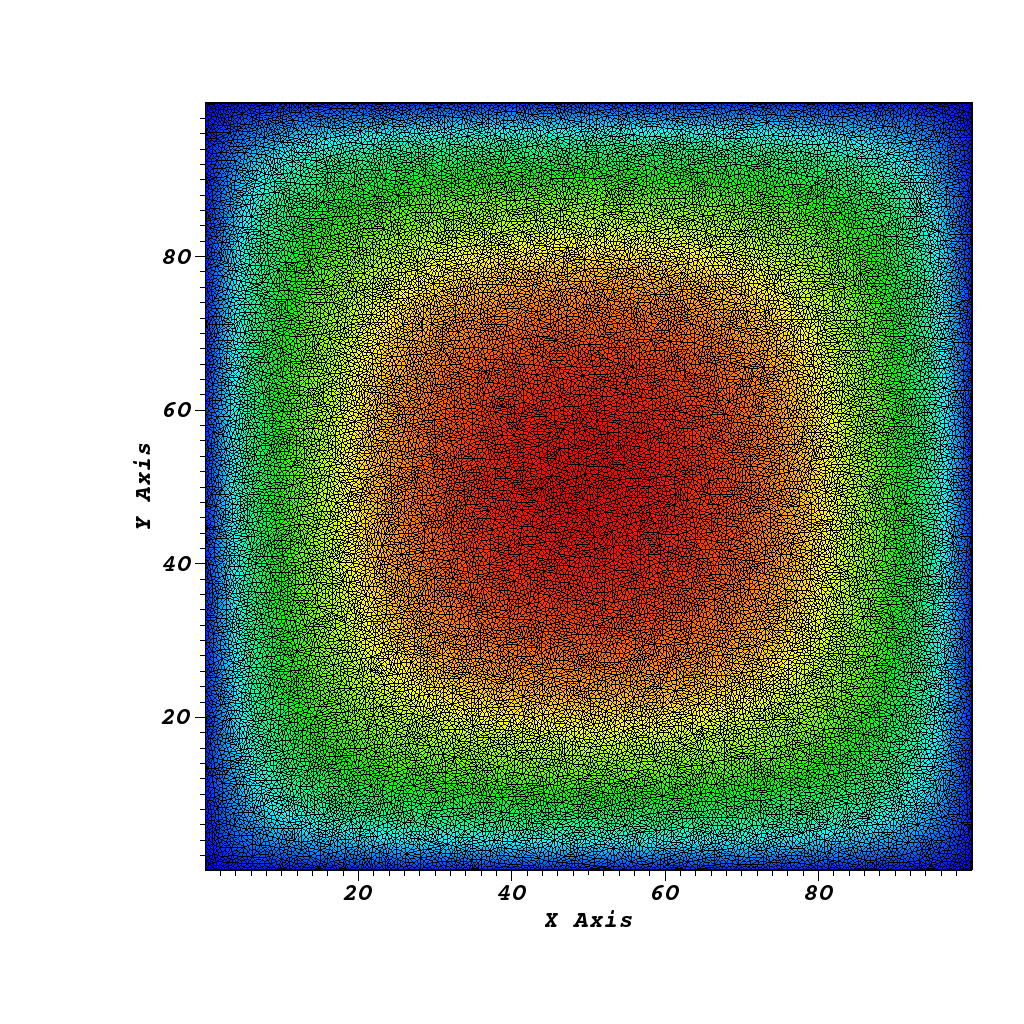
\includegraphics[width=\textwidth]{quad_solu0000}
    \caption{Whole domain}
  \end{subfigure}
  \begin{subfigure}{0.45\textwidth}
    \centering
    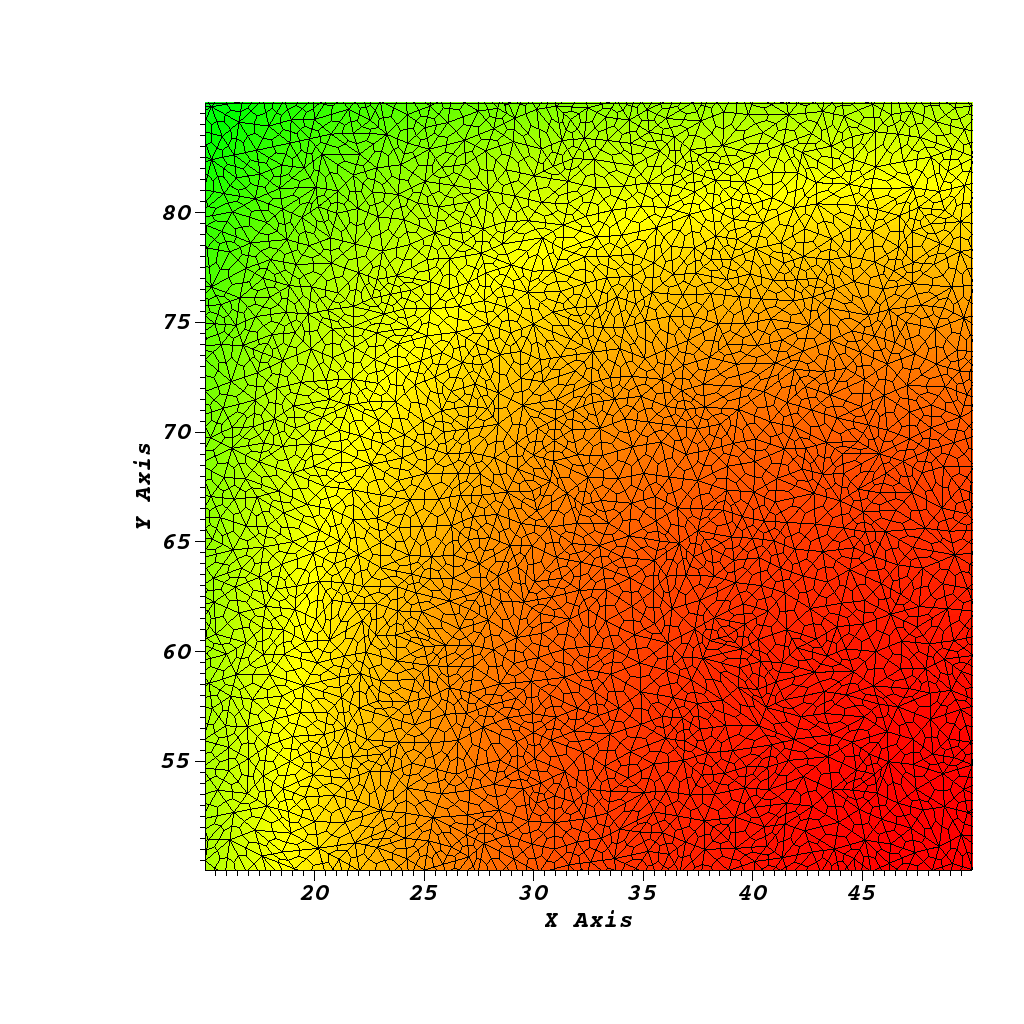
\includegraphics[width=\textwidth]{quad_solu0001}
    \caption{Zoom}
  \end{subfigure}
  \caption{Grids and scalar flux solutions for the homogenous test problem using quadrilateral cells.}
  \label{homog_test_quads}
\end{figure}

\begin{figure}[!htbp]
  \centering
  \begin{subfigure}{0.45\textwidth}
    \centering
    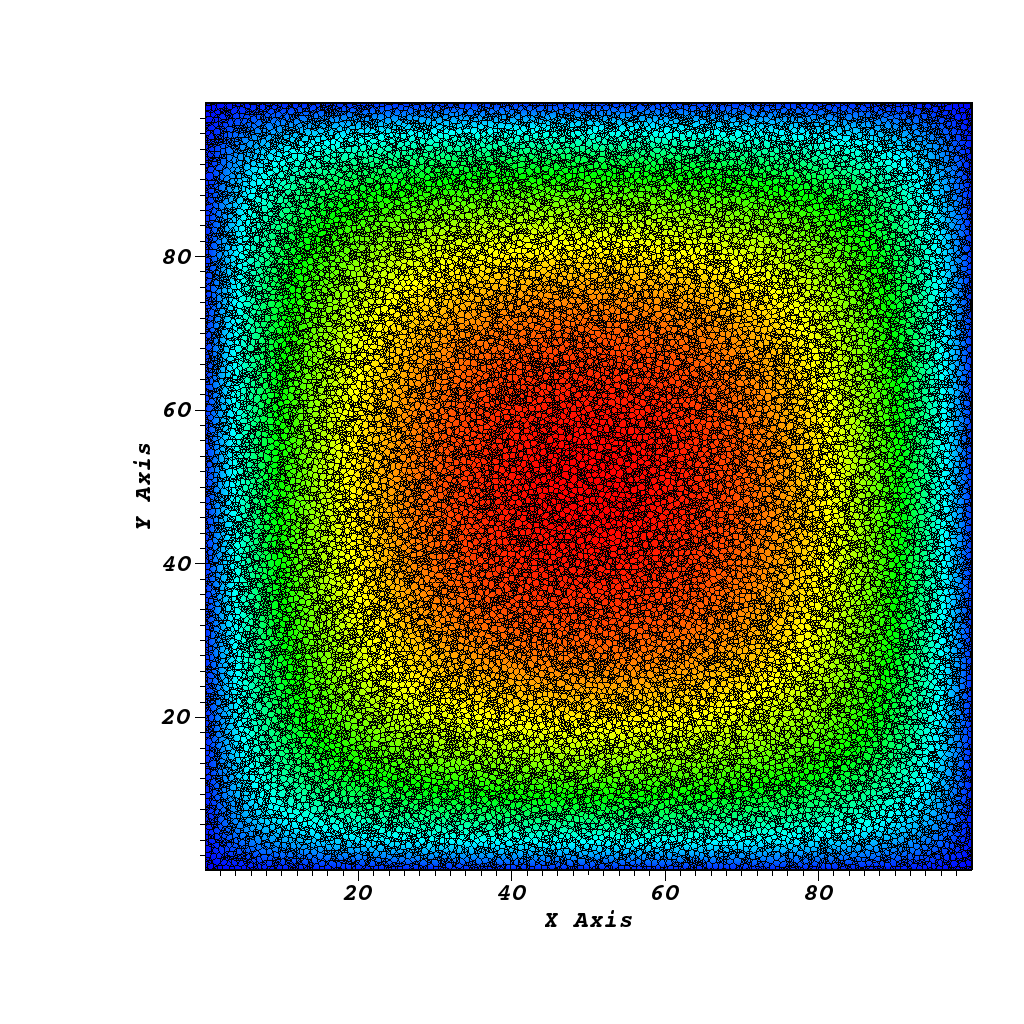
\includegraphics[width=\textwidth]{poly_solu0000}
    \caption{Whole domain}
  \end{subfigure}
  \begin{subfigure}{0.45\textwidth}
    \centering
    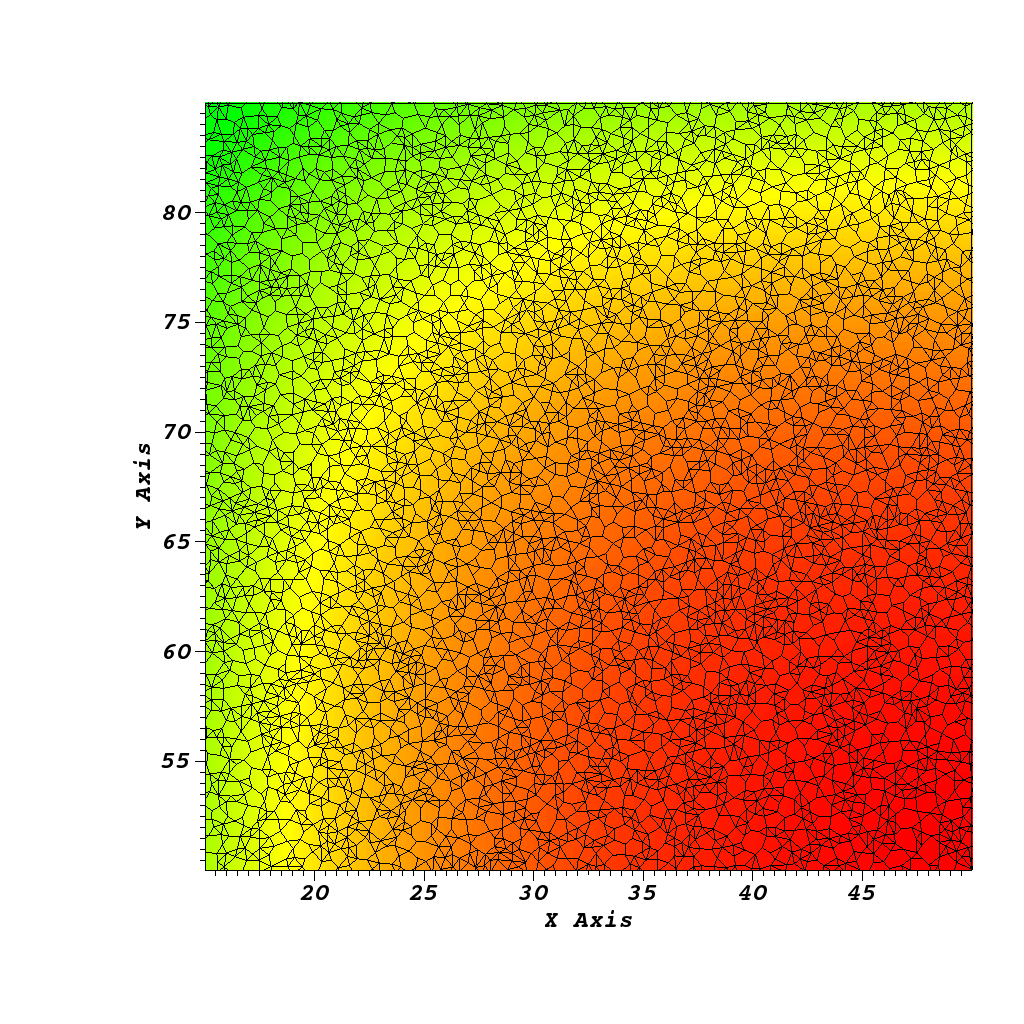
\includegraphics[width=\textwidth]{poly_solu0001}
    \caption{Zoom}
  \end{subfigure}
  \caption{Grids and scalar flux solutions for the homogenous test problem  using arbitrary polygonal cells.}
  \label{homog_test_polys}
\end{figure}

%
%\begin{figure}[!htbp]
  %\centering
  %\begin{subfigure}{0.75\textwidth}
    %\centering
    %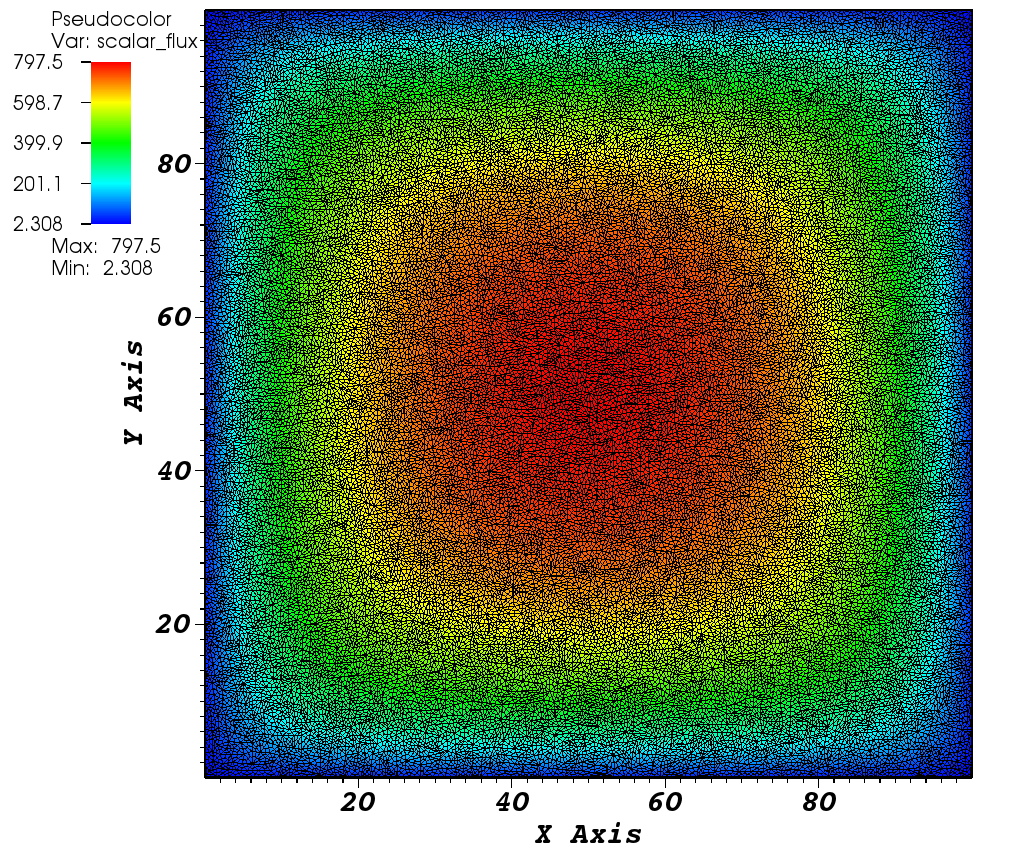
\includegraphics[width=\textwidth]{big_homog_quad_crop}
    %\caption{Quadrilateral cells}
  %\end{subfigure}
  %\begin{subfigure}{0.75\textwidth}
    %\centering
    %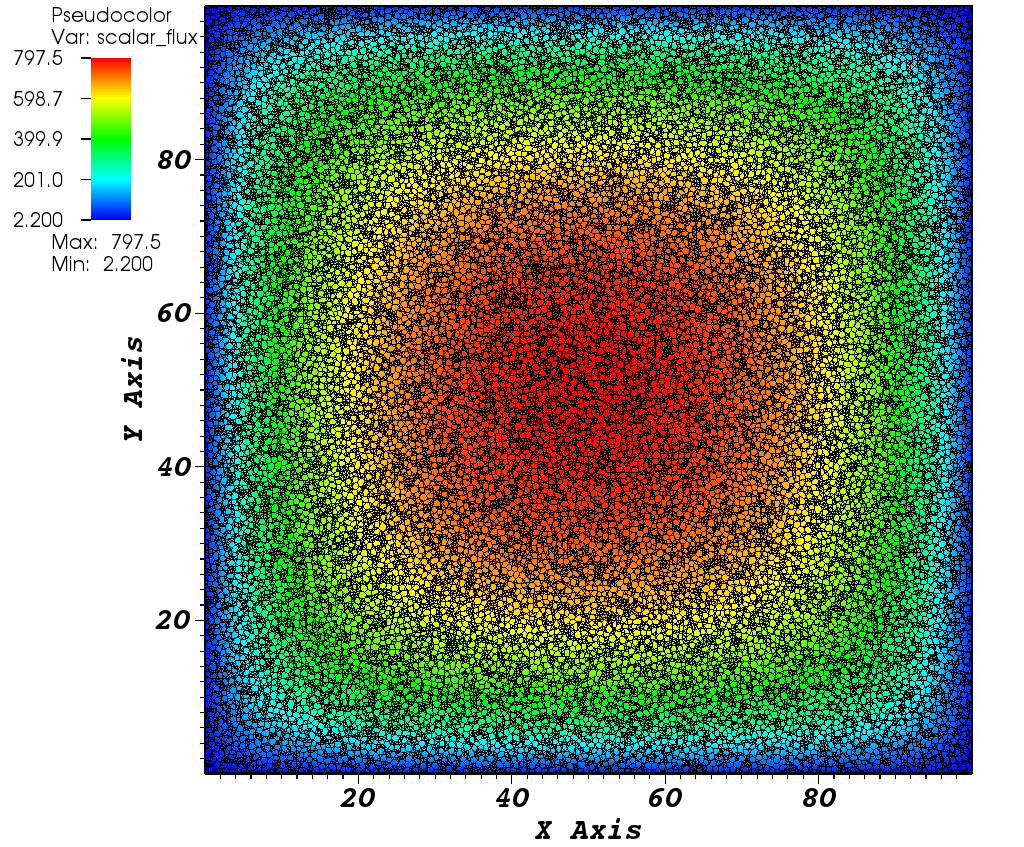
\includegraphics[width=\textwidth]{big_homog_poly_crop}
    %\caption{Polygonal cells}
  %\end{subfigure}
  %\caption{Grids and scalar flux solutions for the homogenous material test problem}
  %\label{homog_test}
%\end{figure}
%
\begin{table}[!htbp]
  \begin{center}
    \caption{Comparison of different preconditioners for the homogeneous test problem (quadrilateral cells).}
    \begin{tabular}{|c|c|c|c|c|c|c|}
      \hline
      & No-DSA & CG & PCG-SGS & PCG-ML/U & PCG-ML/MIS & AGMG \\
      \hline
      SI iterations   & 7311    & 24      & 24       & 24      & 24      & 24 \\
   %Precond init (s)   & NA      & NA      & 0.171358 & 1.8255  & 9.56078 & 0.332 \\
%MIP calculation (s)   & NA      & 1095.7  & 1311.76  & 192.622 & 197.632 & 29.9727 \\
      CG iterations   & NA      & 56649   & 17332    & 630     & 604     & 578 \\
%Total calculation (s) & 39176.7 & 1264.98 & 1477.95  & 363.202 & 367.841 &  194.568 \\
      \hline
    \end{tabular}
    \label{comparison_homog_quad}
  \end{center}
\end{table}
%
\begin{table}[!htbp]
  \begin{center}
    \caption{Comparison of different preconditioners for the homogeneous test problem (polygonal cells).}
    \begin{tabular}{|c|c|c|c|c|c|c|}
      \hline
      & No-DSA & CG & PCG-SGS & PCG-ML/U & PCG-ML/MIS & AGMG \\
      \hline
      SI iterations   & 7311    & 23      & 23      & 23      & 23      & 23 \\
   %Precond init (s)   & NA      & NA      & 0.06388 & 1.73379 & 8.0426  & 0.388 \\
%MIP calculation (s)   & NA      & 877.861 & 1263.31 & 198.63  & 191.989 &
      %31.242 \\
      CG iterations   & NA      & 46262   & 16712   & 652     & 603     & 555 \\
%Total calculation (s) & 42666.7 & 1060.53 & 1447.53 & 382.275 & 384.422 & 216.946 \\
      \hline
    \end{tabular}
    \label{comparison_homog_poly}
  \end{center}
\end{table}

\subsubsection{Test Case with Heterogeneous Media}
%%%%%%%%%%%%%%%%%%%%%%%%%%%%%%%%%%%%%%%%%%%%%%%%%%%%%%%%%%%%%%%%%%%%%%%%%%%%%%%%%%

In this example, a heterogeneous geometry with three materials is used. It is 
composed of 184 triangles, 3,720 quadrilaterals, and 2,791 regular hexagons of 
side $0.05cm$ for a total of 6,695 cells and 32,178 degrees of freedom. 
The domain is $5.28275cm$ by $4.6cm$. 
Reflective boundary conditions are used. A $S_{16}$ angular 
quadrature is used. The SI solver has a relative tolerance of 
$10^{-8}$, and the relative tolerance for MIP-DSA is $10^{-10}$. Figure~\ref {hex_zones}
shows the problem geometry and the material properties are in given
Table~\ref {hex_prop}.
The different linear solvers for MIP-DSA are compared in Table~\ref {comparison_hex}.
%
\begin{figure}[!htbp]
  \centering
  \begin{subfigure}{0.45\textwidth}
    \centering
    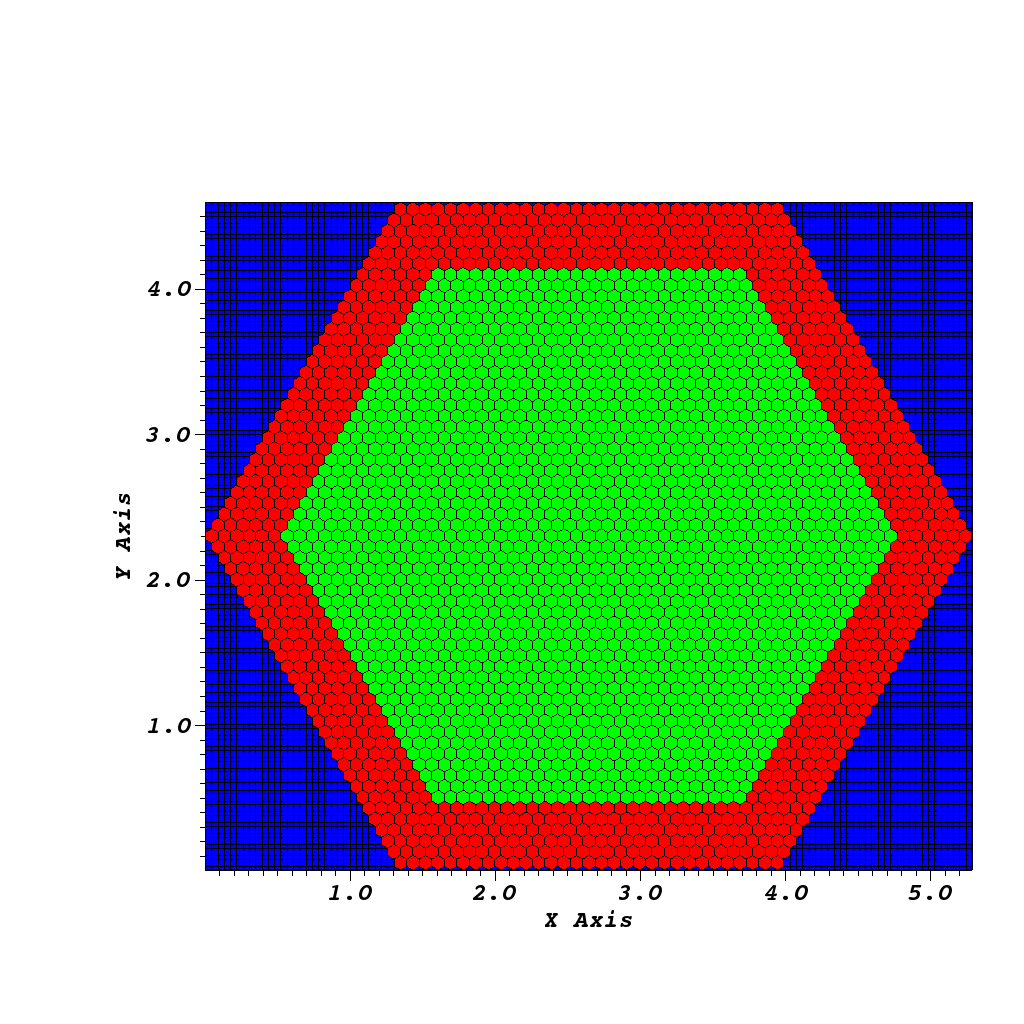
\includegraphics[width=\textwidth]{hexa_grid0000}
    \caption{Whole domain mesh}
  \end{subfigure}
  \begin{subfigure}{0.40\textwidth}
    \centering
    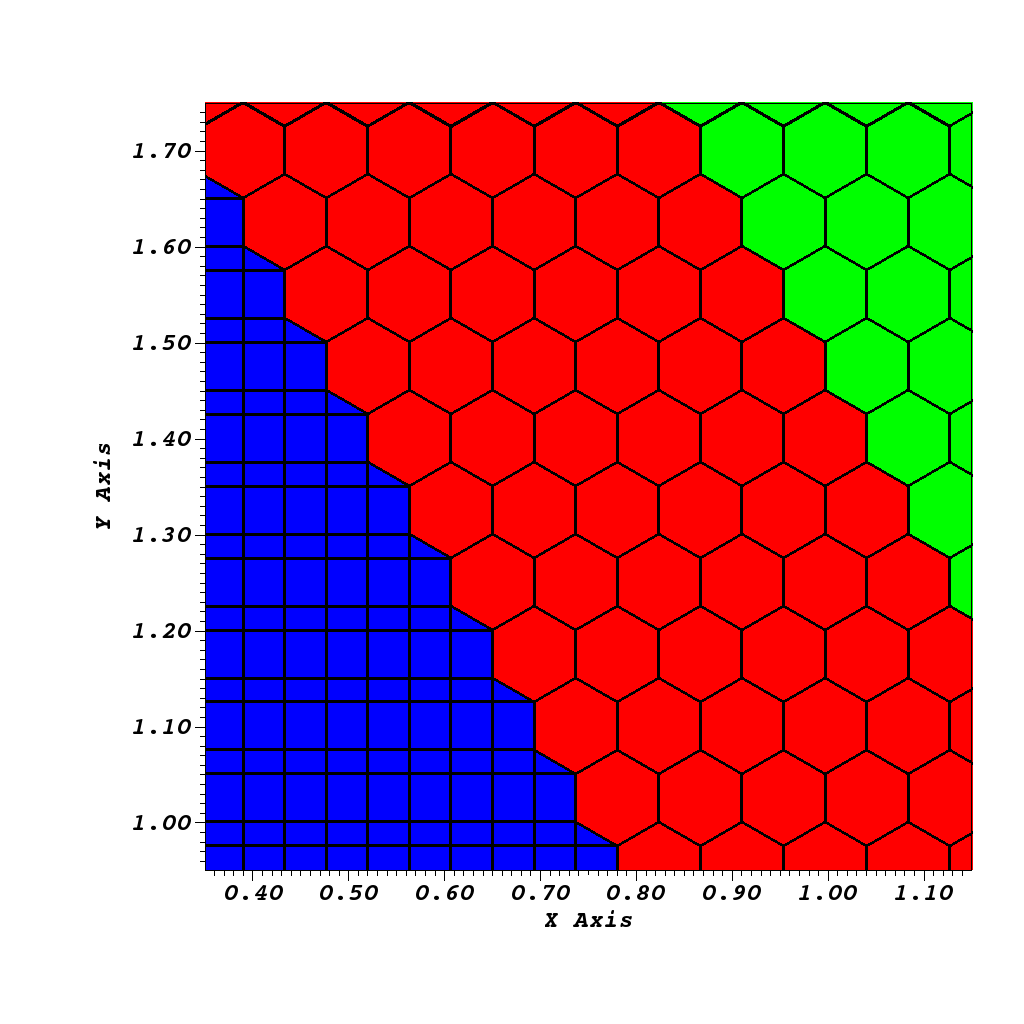
\includegraphics[width=\textwidth]{hexa_grid0001}
    \caption{Zoom}
  \end{subfigure}
  \caption{Material Zones for the Heterogeneous Test Problem}
  \label{hex_zones}
\end{figure}
%
\begin{table}[!htbp]
  \begin{center}
    \caption{Material Properties For the Different Regions of the Heterogeneous Test Problem}
    \begin{tabular}{|c|c|c|c|}
      \hline
       & Inner region & Intermediate region & Outer region \\ \hline
      $\Sigma_t$ $(cm^{-1}) $ & 1.5 & 1.0 & 1.0 \\
      $\Sigma_s$ $(cm^{-1}) $ & 1.4999 & 0.999 & 0.3 \\
     source $(cm^{-3}s^{-1})$ & 1.0 & 0.0 & 0.0 \\
      \hline
    \end{tabular}
    \label{hex_prop}
  \end{center}
\end{table}
%
%
\begin{table}[!htbp]
  \begin{center}
    \caption{Preconditioners Comparison (Heterogeneous Problem).}
    \begin{tabular}{|c|c|c|c|c|c|c|}
      \hline
      & No-DSA & CG & PCG-SGS & PCG-ML/U & PCG-ML/MIS & AGMG\\
      \hline
      SI iterations & 278     & 17      & 17        & 17       & 17      & 17  \\
   %Precond init (s) & NA      & NA      & 0.0160661 & 0.368768 & 1.41632 &
      %0.07  \\
%MIP calculation (s) & NA      & 58.422  & 126.93    & 33.2225  & 31.3045 &
      %2.924 \\
      CG iterations & NA      & 12214   & 6679      & 415      & 386     & 248  \\
%Total calculation (s) & 910.566 & 120.889 & 190.413 & 99.7524  & 97.4666 &
      %70.6424 \\      
      \hline
    \end{tabular}
    \label{comparison_hex}
  \end{center}
\end{table}
%
The remarks made in Section~\ref {sec_homog} for the homogeneous test problem
remain mostly unchanged. MIP-DSA is effective for this heterogeneous test case, and AGMG is
again the most efficient preconditioner. It is interesting to note that, contrary to the
homogeneous tests where the number of CG iterations was about identical  for all
algebraic multigrid preconditioners, in this heterogeneous test case, AGMG requires
significantly fewer iterations than both Trilinos implementations, PCG-ML/U and PCG-ML/MIS.

\subsubsection{Test Case with Locally Refined Cells}
%%%%%%%%%%%%%%%%%%%%%%%%%%%%%%%%%%%%%%%%%%%%%%%%%%%%%%%%%%%%%%%%%%%%%%%%%%%%%%%%%%

In this example, a 3-material domain of size $10cm\times 10cm$ is used. 
Figure~\ref {mat_amr} shows the material zoning and the mesh used. 
The bottom and left sides of the domain have reflective boundary conditions, while the other 
two sides have vacuum boundary conditions. Material properties 
are given in Table~\ref {prop_amr}.

The grid used mimics meshes obtained via adaptive mesh
refinement: the rectangular cells at the interfaces between two materials are refined once more,
leading to a grid composed of 10,482 quadrilaterals, 236 pentagons,
and 2 hexagons for a total of 10,720 cells and 43120 degrees of freedom. 
The distribution of cells is given in Figure~\ref {fig_pol_dist}.


A $S_{16}$ angular quadrature is employed. The tolerance on SI is $10^{-8}$, and
the tolerance on the CG solvers is $10^{-10}$.
The different linear solvers for MIP-DSA are compared in Table~\ref {table_amr}.
%
The conclusions drawn from this test case are similar to the ones made for 
our previous tests. This test case demonstrates that degenerate polygons 
(here, pentagons and hexagons) do not seem to affect the MIP-DSA acceleration.


\begin{figure}[!htbp]
  \centering
  \begin{subfigure}{0.45\textwidth}
    \centering
    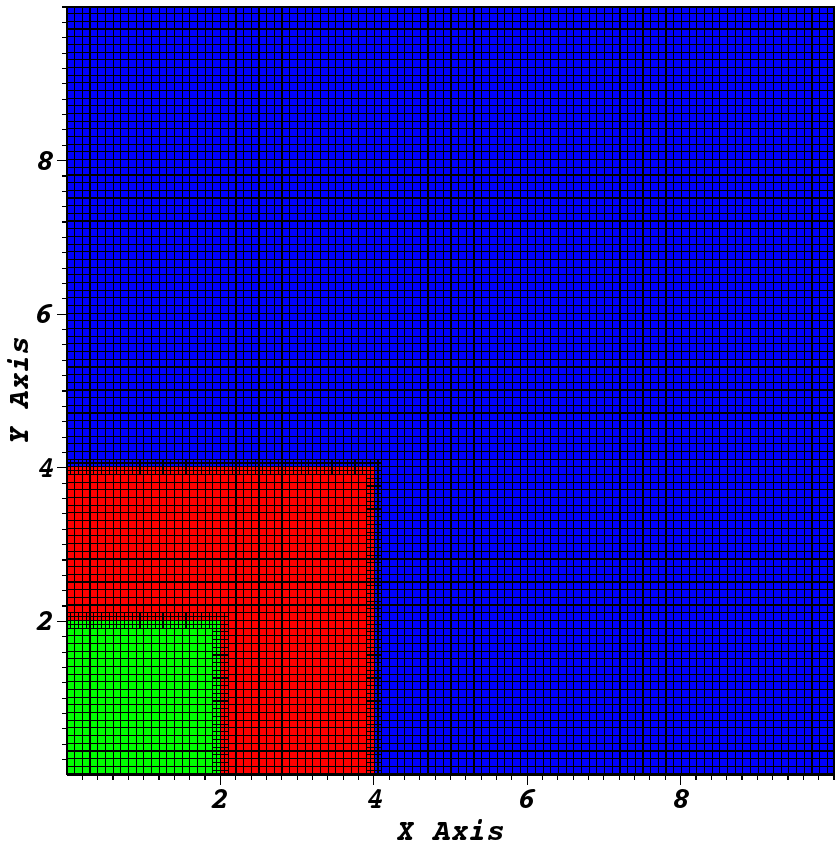
\includegraphics[width=5cm]{zone_amr}
    \caption{Material regions}
    \label{mat_amr}
  \end{subfigure}
  \begin{subfigure}{0.53\textwidth}
    \centering
    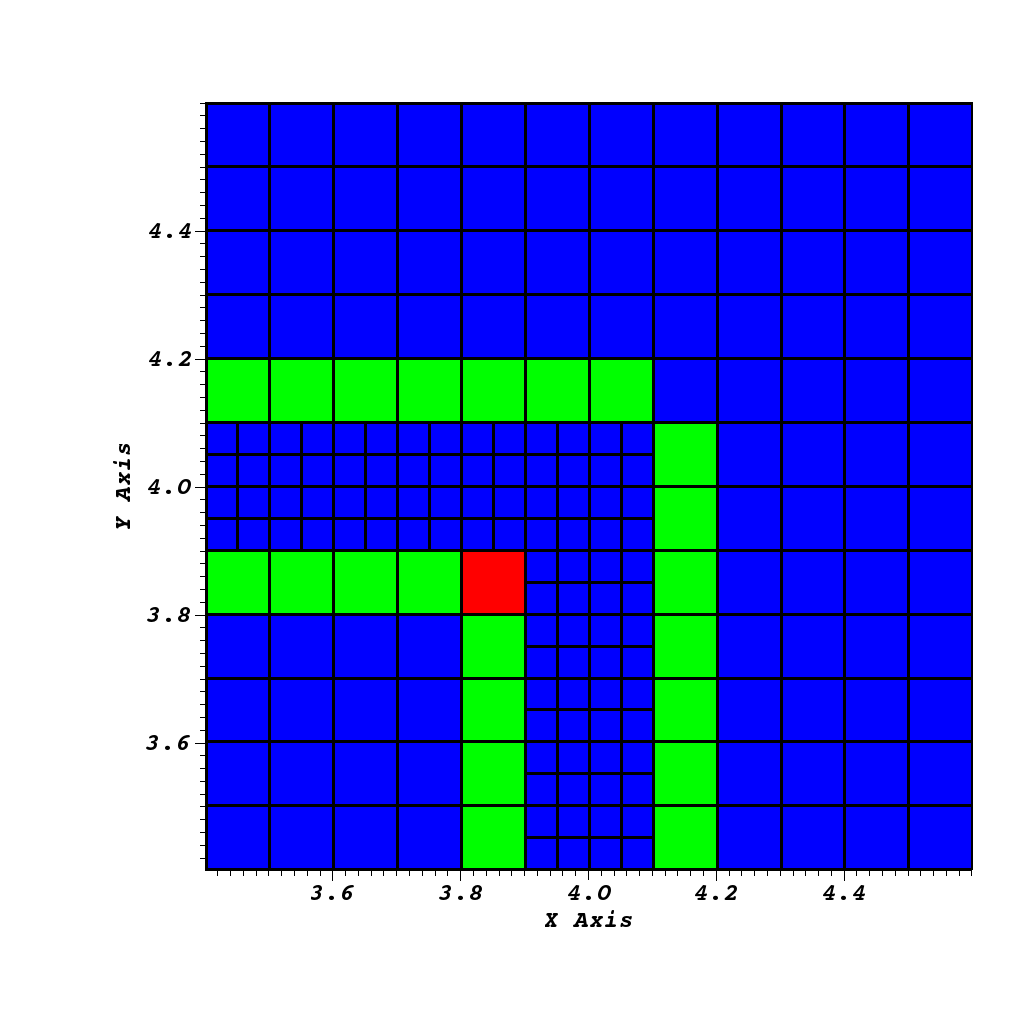
\includegraphics[width=5cm]{amr_grid0001}
    \caption{Polygons distribution (zoom): quadrilaterals (blue cells),  pentagons (green cells),  hexagons (red cells)}
    \label{fig_pol_dist}
  \end{subfigure}
  \caption{AMR-like test domain}
\end{figure}
%
\begin{table}
  \begin{center}
    \caption{Material Properties (AMR-like Problem)}
    \begin{tabular}{|c|c|c|c|}
      \hline
      & Inner region & Intermediate region & Outer region  \\ \hline
    $\Sigma_t$ $(cm^{-1})$ & 1.5  & 1.0 & 1.0 \\
    $\Sigma_s$ $(cm^{-1})$ & 1.44 & 0.9 & 0.3 \\
  Source $(cm^{-3}s^{-1})$ & 1.0  & 0.0 & 0.0 \\
      \hline
    \end{tabular}
    \label{prop_amr}
  \end{center}
\end{table}

\begin{table}[H]
  \caption{Preconditioners Comparison for the AMR Mesh}
  \begin{center}
    \begin{tabular}{|c|c|c|c|c|c|c|}
      \hline
       & No-DSA & CG & PCG-SGS & PCG-ML/U & PCG-ML/MIS & AGMG \\
      \hline
   SI iterations & 184     & 19      & 19       & 19      & 19       & 19 \\
%Precond init (s) & NA      & NA      & 0.043463 & 0.358002 & 1.19301 & 0.0111\\
%MIP calculation (s) & NA   & 48.1908 & 81.0992  & 25.2699 & 25.0699  & 
      %2.56198\\
   CG iterations & NA      & 11300   & 4734     & 361     & 361      & 264 \\
     %Total calculation (s) & 802.985 & 138.825 & 172.423  & 116.018 & 116.517  &  94.1963\\
      \hline
    \end{tabular}
    \label{table_amr}
  \end{center}
\end{table}

\subsubsection{Test Cases High Aspect Ratio Grids}
%%%%%%%%%%%%%%%%%%%%%%%%%%%%%%%%%%%%%%%%%%%%%%%%%%%%%%%%%%%%%%%%%%%%%%%%%%%%%%%%%%

In these last two examples, a square domain  of $100cm \times 100cm$ with vacuum boundaries
is employed. There are 10,000 cells (thus, 40,000 degrees of freedom). Again, the relative 
tolerance on SI is $10^{-8}$ and the relative tolerance for CG is $10^{-10}$. 
An $S_8$ GLC angular quadrature is used. $\Sigma_t = 1cm^{-1}$, $\Sigma_s = 0.999cm^{-1}$
and the source is $1n/(cm^3s)$. 
In the first run, the domain is discretized using 100 subdivisions of the $x$ and $y$
axes, i.e., 10,000 square cells with an aspect ratio of one. In the second run, 
the domain is discretized using 1,000 subdivision along $x$ and 10 along $y$ 
(the aspect ratio is then 100).
%
As expected, solving the MIP-DSA equations requires more CG iterations when the aspect
ratio increases. PCG-ML/U and PCG-ML/MIS are significantly more affected by the
increase in the aspect ratio than the other methods. AGMG is the least
affected by the change of aspect ratio and is again the best performing
preconditioner.
%
\begin{table}[!htbp]
  \caption{Preconditioners Comparison for a Rectangular Grid with an Aspect Ratio of 1}
  \begin{center}
    \begin{tabular}{|c|c|c|c|c|c|c|}
      \hline
       & No-DSA & CG & PCG-SGS & PCG-ML/U & PCG-ML/MIS & AGMG \\
      \hline
      SI iterations & 7311      & 21      & 21      & 21       & 21      & 21 \\
   %Precond init (s) & NA        & NA      & 0.01422 & 0.051373 & 1.13144 &
      %0.044 \\
%MIP calculation (s) & NA        & 32.3825 & 73.8422 & 24.0707  & 25.0065 &
      %1.7114 \\
      CG iterations & NA        & 8363    & 4853    & 376      & 375     &
      221\\
%Total calculation (s) & 7356.96 & 56.8993 & 98.2609 & 50.1247  & 51.5396 &
      %25.9306 \\
      \hline
    \end{tabular}
    \label{table_ar_1}
  \end{center}
\end{table}
%
\begin{table}[!htbp]
  \caption{Preconditioners Comparison for a Rectangular Grid with an Aspect Ratio of 100}
  \begin{center}
    \begin{tabular}{|c|c|c|c|c|c|c|}
      \hline
       & No-DSA & CG & PCG-SGS & PCG-ML/U & PCG-ML/MIS & AGMG \\
      \hline
      SI iterations & 7304    & 24      & 24        & 24       & 24      & 24 \\
   %Precond init (s) & NA      & NA      & 0.0164239 & 0.362463 & 1.03128 & 0.052 \\
%MIP calculation (s) & NA      & 372.227 & 742.902   & 941.06   & 922.258 &
      %6.93176 \\
      CG iterations & NA      & 84802   & 43466     & 14180    & 13896   & 821 \\
%Total calculation (s) & 9035.6 & 414.301 & 784.77   & 985.796  & 966.77  &
      %44.7032 \\
      \hline
    \end{tabular}
    \label{table_ar_100}
  \end{center}
\end{table}                  
%%%%%%%%%%%%%%%%%%%%%%%%%%%%%%%%%%%%%%%%%%%%%%%%%%%%%%%%%%%%%%%%%%%%%%%%%%%%%%%%%%%%%%%%%%%%%%%%%%%%%%%%%%%
%%%%%%%%%%%%%%%%%%%%%%%%%%%%%%%%%%%%%%%%%%%%%%%%%%%%%%%%%%%%%%%%%%%%%%%%%%%%%%%%%%%%%%%%%%%%%%%%%%%%%%%%%%%

%%%%%%%%%%%%%%%%%%%%%%%%%%%%%%%%%%%%%%%%%%%%%%%%%%%%%%%%%%%%%%%%%%%%%%%%%%%%%%%%%%%%%%%%%%%%%%%%%%%%%%%%%%%
%%%%%%%%%%%%%%%%%%%%%%%%%%%%%%%%%%%%%%%%%%%%%%%%%%%%%%%%%%%%%%%%%%%%%%%%%%%%%%%%%%%%%%%%%%%%%%%%%%%%%%%%%%%
%%%%%%%%%%%%%%%%%%%%%%%%%%%%%%%%%%%%%%%%%%%%%%%%%%%%%%%%%%%%%%%%%%%%%%%%%%%%%%%%%%
%%%%%%%%%%%%%%%%%%%%%%%%%%%%%%%%%%%%%%%%%%%%%%%%%%%%%%%%%%%%%%%%%%%%%%%%%%%%%%%%%%
\section{Conclusions} \label{sec_conc}
%%%%%%%%%%%%%%%%%%%%%%%%%%%%%%%%%%%%%%%%%%%%%%%%%%%%%%%%%%%%%%%%%%%%%%%%%%%%%%%%%%
%%%%%%%%%%%%%%%%%%%%%%%%%%%%%%%%%%%%%%%%%%%%%%%%%%%%%%%%%%%%%%%%%%%%%%%%%%%%%%%%%%
We have extended the Modified Interior Penalty (MIP) form of Diffusion Synthetic Acceleration (DSA) 
to \sn radiation transport solves performed on arbitrary polygonal grids discretized 
with Piece-Wise Linear Discontinuous finite elements. 
The MIP-DSA equation employs the same discontinuous finite element trial spaces as 
the spatial discretization of the \sn transport equation. As such, 
%Since this DSA employs the same discontinuous finite element spaces as the \sn transport discretization,
only a few additional elementary matrices need to be implemented to an existing \sn code. 
%We proposed a simple way to compute the penalty coefficient on such grids. 
%
%%Numerical tests have been run on different grids with various types of polygonal cells,
%%demonstrating the effectiveness of MIP as a diffusion synthetic accelerator for 
%%\sn transport on arbitrary polygonal grids.
%
%. The advantage of is the potential 
%reduction of the numbers of unknowns and the possibility to use adaptive mesh 
%refinement without having hanging nodes. 
%

Fourier analyses show that the PWLD discretization of the MIP diffusion synthetic accelerator 
is stable and effective, including for cells with high-aspect ratios. 
%
Numerical experiments have been performed with grids containing various types of polygonal cells
(random quadrilaterals, random polygons), including
grids with different polygon types for a given mesh and tests with degenerate polygons that mimic
grids obtained in adaptive mesh refinement strategies. In these tests, MIP-DSA always performed effectively,
reducing significantly the number of Source Iterations needed for convergence. 
We noted that the effectiveness of MIP does not seem to be affected by the meshes employed. 
%

The MIP-DSA  matrix is Symmetric Positive Definite (SPD) and we solved the resulting linear system 
of equations using a standard Conjugate Gradient method with different preconditioners. 
Algebraic multigrid techniques (AGMG and ML) were found to be the most
effective preconditioner.% with AGMG 
%being more than 20 times faster than unpreconditioned CG.

We conclude that MIP-DSA is an effective alternative to
carry out diffusion synthetic accelerations for \sn radiation transport problems on arbitrary polygonal grids and 
grids obtained through mesh adaptivity.
Future extensions of this work will include the implementation of the MIP-DSA equations in a 3D parallel \sn code.

% and full integration with   



%%%%%%%%%%%%%%%%%%%%%%%%%%%%%%%%%%%%%%%%%%%%%%%%%%%%%%%%%%%%%%%%%%%%%%%%%%%%%%%%%%%%%%%%%%%%%%%%%%%%%%%%%%%
%%%%%%%%%%%%%%%%%%%%%%%%%%%%%%%%%%%%%%%%%%%%%%%%%%%%%%%%%%%%%%%%%%%%%%%%%%%%%%%%%%%%%%%%%%%%%%%%%%%%%%%%%%%

%\textcolor{red}{Is this appendix needed?}
%\appendix
\section{Building the mass matrix}
Let us take for example the mass matrix $M_{PWLD}$ and the mass matrix on a
``side'' sub-cell $M$. We assume that the third basis function is associated
to the middle point of the PWLD cell. The first (respectively second) basis function
on the cell correspond to the first (respectively second) basis function of
the ``side'' sub-cell.

{\allowdisplaybreaks
\begin{align}
& M_{PWLD}(0,0) = M_{PWLD}(0,0) + M(0,0) + \alpha M(0,2) + \alpha M(2,0) + 
\alpha^2M(2,2)\\
& M_{PWLD}(0,1) = M_{PWLD}(0,1) + M(0,1) + \alpha M(0,2) + \alpha M(2,1) + 
\alpha^2M(2,2)\\
& M_{PWLD}(0,2) = M_{PWLD}(0,2) + \alpha M(0,2) + \alpha^2 M(2,2)\\
& M_{PWLD}(0,3) = M_{PWLD}(0,3) + \alpha M(0,2) + \alpha^2M(2,2)\\
& M_{PWLD}(1,0) = M_{PWLD}(1,0) + M(1,0) + \alpha M(1,2) + \alpha M(2,0) + 
\alpha^2M(2,2)\\
& M_{PWLD}(1,1) = M_{PWLD}(1,1) + M(1,1) + \alpha M(1,2) + \alpha M(2,1) + 
\alpha^2M(2,2)\\
& M_{PWLD}(1,2) = M_{PWLD}(1,2) + \alpha M(1,2) + \alpha^2M(2,2)\\
& M_{PWLD}(1,3) = M_{PWLD}(1,3) + \alpha M(1,2) + \alpha^2M(2,2)\\
& M_{PWLD}(2,0) = M_{PWLD}(2,0) + \alpha M(2,0) + \alpha^2M(2,2)\\
& M_{PWLD}(2,1) = M_{PWLD}(2,1) + \alpha M(2,1) + \alpha^2M(2,2)\\
& M_{PWLD}(2,2) = M_{PWLD}(2,2) + \alpha^2M(2,2)\\
& M_{PWLD}(2,3) = M_{PWLD}(2,3) + \alpha^2M(2,2)\\
& M_{PWLD}(3,0) = M_{PWLD}(3,0) + \alpha M(2,0) + \alpha^2M(2,2)\\
& M_{PWLD}(3,1) = M_{PWLD}(3,1) + \alpha M(2,1) + \alpha^2M(2,2)\\
& M_{PWLD}(3,2) = M_{PWLD}(3,2) + \alpha^2M(2,2)\\
& M_{PWLD}(3,3) = M_{PWLD}(3,3) + \alpha^2M(2,2)
\end{align}}    
The mass matrix $M$ is given by:
\begin{equation}
M = \frac{A}{12}
\begin{pmatrix}
2 & 1 & 1\\
1 & 2 & 1\\
1 & 1 & 2
\end{pmatrix}
\end{equation}
where $A$ is the area of the ``side'' sub-cell.


% bibliography
\bibliographystyle{unsrt}
\bibliography{biblio}

\end{document}

